% This file was created (at least in part) by the script ParseMdtoLatex by Louis du Plessis
% (Available from https://github.com/taming-the-beast)

\documentclass[11pt]{article}
%%%%%%%%%%%%%%%%%%%%%%%%%%%%%%%%%%%%%%%%%%%%%%%%%%%%%%%%%%%%%%%
% DO NOT EDIT THIS FILE UNLESS YOU KNOW WHAT YOU ARE DOING!!! %
%%%%%%%%%%%%%%%%%%%%%%%%%%%%%%%%%%%%%%%%%%%%%%%%%%%%%%%%%%%%%%%

\usepackage[]{authblk}
\usepackage{graphicx}
\usepackage{color}
\usepackage{longtable}
\usepackage{hanging}
\usepackage{indentfirst}
\usepackage{setspace}
\usepackage{enumitem}
\usepackage{verbatim}
\usepackage{upgreek}
\usepackage{framed}
\usepackage{textcomp}
\usepackage{url}
\usepackage{soul}
\usepackage{amsmath, amsfonts,amssymb,mathrsfs}
\usepackage{fancyhdr}
\usepackage[compact]{titlesec}
\usepackage[T1]{fontenc}
\usepackage{lmodern}

\usepackage[backend=bibtex,hyperref=true,citestyle=authoryear,bibstyle=authortitle,firstinits=true,terseinits=true,doi=false,url=false,eprint=false,maxbibnames=10,maxcitenames=2]{biblatex}
\DeclareCiteCommand{\cite}
  {\usebibmacro{prenote}}
  {\usebibmacro{citeindex}%
   \printtext[bibhyperref]{\usebibmacro{cite}}}
  {\multicitedelim}
  {\usebibmacro{postnote}}

\DeclareCiteCommand*{\cite}
  {\usebibmacro{prenote}}
  {\usebibmacro{citeindex}%
   \printtext[bibhyperref]{\usebibmacro{citeyear}}}
  {\multicitedelim}
  {\usebibmacro{postnote}}

\DeclareCiteCommand{\parencite}[\mkbibparens]
  {\usebibmacro{prenote}}
  {\usebibmacro{citeindex}%
    \printtext[bibhyperref]{\usebibmacro{cite}}}
  {\multicitedelim}
  {\usebibmacro{postnote}}

\DeclareCiteCommand*{\parencite}[\mkbibparens]
  {\usebibmacro{prenote}}
  {\usebibmacro{citeindex}%
    \printtext[bibhyperref]{\usebibmacro{citeyear}}}
  {\multicitedelim}
  {\usebibmacro{postnote}}

\DeclareCiteCommand{\footcite}[\mkbibfootnote]
  {\usebibmacro{prenote}}
  {\usebibmacro{citeindex}%
  \printtext[bibhyperref]{ \usebibmacro{cite}}}
  {\multicitedelim}
  {\usebibmacro{postnote}}

\DeclareCiteCommand{\footcitetext}[\mkbibfootnotetext]
  {\usebibmacro{prenote}}
  {\usebibmacro{citeindex}%
   \printtext[bibhyperref]{\usebibmacro{cite}}}
  {\multicitedelim}
  {\usebibmacro{postnote}}

\DeclareCiteCommand{\textcite}
  {\boolfalse{cbx:parens}}
  {\usebibmacro{citeindex}%
   \printtext[bibhyperref]{\usebibmacro{textcite}}}
  {\ifbool{cbx:parens}
     {\bibcloseparen\global\boolfalse{cbx:parens}}
     {}%
   \multicitedelim}
  {\usebibmacro{textcite:postnote}}

\newcommand{\citep}{\parencite}
\newcommand{\citet}{\textcite}
\defbibheading{relevref}[\refname]{\section*{Relevant References}}

\renewcommand{\postnotedelim}{\iffieldpages{postnote}{\addcolon}{\addcomma\space}} 
\DeclareFieldFormat{postnote}{#1} 

\DeclareFieldFormat[article, inbook, incollection, inproceedings, patent, thesis, unpublished]{title}{#1}
\DeclareFieldFormat[article, inbook, incollection, inproceedings, patent, thesis, unpublished]{journaltitle}{\mkbibemph{#1}\nopunct}
\DeclareFieldFormat[article, inbook, incollection, inproceedings, patent, thesis, unpublished]{volume}{{#1}\addcolon} %puts volume number in parens
%\DeclareFieldFormat[article, inbook, incollection, inproceedings, patent, thesis, unpublished]{year}{\mkbibparens{#1}\nopunct} %puts year in parens

\DeclareFieldFormat[article, incollection, patent, thesis, unpublished]{pages}{{\nopp#1}}

\DeclareFieldFormat{sentencecase}{\MakeSentenceCase{#1}}

\renewbibmacro*{title}{%
  \ifthenelse{\iffieldundef{title}\AND\iffieldundef{subtitle}}
    {}
    {\ifthenelse{\ifentrytype{article}\OR\ifentrytype{inbook}%
      \OR\ifentrytype{incollection}\OR\ifentrytype{inproceedings}%
      \OR\ifentrytype{inreference}}
      {\printtext[title]{%
        \printfield[sentencecase]{title}%
        \setunit{\subtitlepunct}%
        \printfield[sentencecase]{subtitle}}}%
      {\printtext[title]{%
        \printfield[titlecase]{title}%
        \setunit{\subtitlepunct}%
        \printfield[titlecase]{subtitle}}}%
     \newunit}%
  \printfield{titleaddon}}

\DefineBibliographyStrings{english}{% various adjustments to common bib entry strings
urlseen = {Accessed:},% What goes in front of the date a URL was accessed/retrieved etc.
editor = {(Ed)},%Ed – no dot, in brackets
editors = {(Eds)},% Eds – no dot, in brackets
byeditor = {(Ed.)}}% ‘Edited by’ for edited works

\DeclareNameAlias{default}{last-first}

\renewbibmacro{in:}{}

\renewbibmacro{publisher+location+date}{
  \iflistundef{publisher}
    {}
    {\printlist{publisher}%
       {\addcomma\space}%
      \iflistundef{location}
        {}
        {\printlist{location}}%
    }
}

\DeclareBibliographyDriver{article}{%
\usebibmacro{bibindex}%
\usebibmacro{begentry}%
\usebibmacro{author/translator+others}%
\newunit\newblock
\printfield{year}%
\setunit{\labelnamepunct}\newblock
\usebibmacro{title}%
\newunit
\printlist{language}%
\newunit\newblock
\usebibmacro{byauthor}%
\newunit\newblock
\usebibmacro{bytranslator+others}%
\newunit\newblock
\printfield{version}%
\newunit\newblock
%\usebibmacro{in:}% %mit in:
\usebibmacro{journal}%
\newunit\newblock
\printfield{volume}%
\newunit\newblock
\usebibmacro{byeditor+others}%
\newunit\newblock
\usebibmacro{note+pages}%
\newunit\newblock
\iftoggle{bbx:isbn}
{}%
\newunit\newblock
\usebibmacro{doi+eprint+url}%
\newunit\newblock
\usebibmacro{addendum+pubstate}%
\newunit\newblock
\usebibmacro{pageref}%
\usebibmacro{finentry}}

\DeclareBibliographyDriver{inproceedings}{%
\usebibmacro{bibindex}%
\usebibmacro{begentry}%
\usebibmacro{author/translator+others}%
\newunit\newblock
\printfield{year}%
\setunit{\labelnamepunct}\newblock
\usebibmacro{title}%
\newunit
\printlist{language}%
\newunit\newblock
\usebibmacro{byauthor}%
\newunit\newblock
\usebibmacro{bytranslator+others}%
\newunit\newblock
\printfield{version}%
\newunit\newblock
%\usebibmacro{in:}% %mit in:
\usebibmacro{booktitle}%
\newunit\newblock
\printfield{volume}%
\newunit\newblock
\usebibmacro{byeditor+others}%
\newunit\newblock
\usebibmacro{publisher+location+date}%
\newunit\newblock
\usebibmacro{note+pages}%
\newunit\newblock
\usebibmacro{pageref}%
\usebibmacro{finentry}}

\DeclareBibliographyDriver{book}{%
\usebibmacro{bibindex}%
\usebibmacro{begentry}%
\usebibmacro{author/translator+others}%
\newunit\newblock
\printfield{year}%
\setunit{\labelnamepunct}\newblock
\usebibmacro{title}%
\newunit
\printlist{language}%
\newunit\newblock
\usebibmacro{byauthor}%
\newunit\newblock
\usebibmacro{bytranslator+others}%
\newunit\newblock
%\usebibmacro{in:}% %mit in:
\usebibmacro{booktitle}%
\newunit\newblock
\printfield{volume}%
\newunit\newblock
\usebibmacro{publisher+location+date}%
\newunit\newblock
\usebibmacro{note+pages}%
\newunit\newblock
\usebibmacro{pageref}%
\usebibmacro{finentry}}




\setlist{nolistsep}

\setlength{\evensidemargin}{0in}
\setlength{\headheight}{0in}
\setlength{\headsep}{0in}
\setlength{\oddsidemargin}{-0.25in}
\setlength{\paperheight}{11in}
\setlength{\paperwidth}{8.5in}
\setlength{\tabcolsep}{0in}
\setlength{\textheight}{9in}
\setlength{\textwidth}{7in}
\setlength{\topmargin}{0in}
\setlength{\topskip}{0in}
\setlength{\voffset}{0in}
\parskip = 0.15in
\pagestyle{plain}
\setlength{\parindent}{0cm}

\definecolor{citescol}{RGB}{194,101,1}
\definecolor{urlscol}{RGB}{0,150,206}
\definecolor{linkscol}{RGB}{149,0,207}
\definecolor{mycol}{RGB}{25,23,191}
\definecolor{outputcol}{RGB}{34,139,34}
\definecolor{tcol}{RGB}{165,0,14}


\DeclareMathAlphabet{\msfsl}{T1}{cmr}{m}{it}
\DeclareMathAlphabet{\msyf}{OMX}{pcr}{m}{it}
\newcommand{\alf}{\upalpha}
\newcommand{\hilight}[1]{\colorbox{yellow}{#1}}

\newcommand{\levelone}[1]{
\bigskip
\noindent{\LARGE{\textsc{#1}}}
\vspace {0.05in}
}

\newcommand{\leveltwo}[1]{
\bigskip
\noindent{\Large{\textit{#1}}}
\vspace {-1mm}
}

\newcommand{\descriptionhead}[1]{
\noindent{\textcolor{mycol}{\textbf{\textit{#1}}}}\\ \vspace{-7mm}
}

\newcommand{\dhead}[1]{
\noindent{\textbf{\textit{#1 --}}}
}



\newcommand{\exs}[1]{
\vspace{-4mm}
\begin{itemize}
\item #1 \\ \vspace{-8mm}
\end{itemize}
}

\newcommand{\nbo}[1]{{\color{red}{#1}}}


\newcommand{\stepbullet}{\noindent \textbullet \ }
\newcommand{\mi}[1]{\textbf{\textit{#1}}}


\newcommand{\levelthree}[1]{\textit{#1 --}}


%\bibliographystyle{apalike}
%\bibpunct[; ]{(}{)}{;}{a}{,}{;}


\usepackage[breaklinks]{hyperref}
\usepackage[all]{hypcap}
\hypersetup{colorlinks=true,linkcolor=linkscol,citecolor=citescol,urlcolor=urlscol}


\newcommand{\R}{\texttt{R} }
\newcommand{\TESS}{\texttt{TESS}}
\newcommand{\PBD}{\texttt{PBD}}
\newcommand{\DDD}{\texttt{DDD}}
\newcommand{\Laser}{\texttt{laser}}
\newcommand{\TreePar}{\texttt{TreePar}}
\newcommand{\diversitree}{\texttt{diversitree}}
\newcommand{\RevBayes}{\texttt{RevBayes}}
\newcommand{\Rev}{\texttt{Rev}}
\newcommand{\MrBayes}{\texttt{MrBayes}}
\newcommand{\BEAST}{\texttt{BEAST}}
\newcommand{\PhyloBayes}{\texttt{PhyloBayes}}
\newcommand{\PAML}{\texttt{PAML}}

\let\otheriint\iint
\let\iint\relax
\usepackage{ wasysym }

\usepackage{framed}
\usepackage[]{listings}
%\usepackage{fontspec}
\usepackage{placeins}
\usepackage{epstopdf}



\lstset{backgroundcolor=\color[rgb]{0.972,0.972,0.972},
		tabsize=4,
		rulecolor=,
        basicstyle=\scriptsize,
        upquote=true,
        aboveskip={1.5\baselineskip},
        columns=fixed,
        showstringspaces=false,
        extendedchars=true,
        breaklines=true,
        prebreak = \raisebox{0ex}[0ex][0ex]{\ensuremath{\hookleftarrow}},
        frame=single,
        showtabs=false,
        showspaces=false,
        showstringspaces=false,
        identifierstyle=\ttfamily,
        keywordstyle=\color[rgb]{0,0,1},
        commentstyle=\color[rgb]{0.133,0.545,0.133},
        stringstyle=\color[rgb]{0.627,0.126,0.941}
}

\definecolor{shadecolor}{RGB}{194,225,255}

\setlength{\tabcolsep}{5pt}
\setlength{\topmargin}{-0.4in}
\setlength{\headheight}{14.5pt}
\pagestyle{fancy}

\newcommand{\taha}[1]{{\textcolor{red}{[TAH comment: #1]}}} % TAH comment

\titlespacing{\section}{0pt}{*0}{*0}
\titlespacing{\subsection}{0pt}{*0}{*0}
\titlespacing{\subsubsection}{0pt}{*0}{*0}

\titleformat{\section}
  {\normalfont\Large\bfseries\color{mycol}}
  {\thesection}{1em}{}

\titleformat{\subsection}
  {\normalfont\large\bfseries\color{mycol}}
  {\thesubsection}{1em}{}

\titleformat{\subsubsection}
  {\normalfont\bfseries\color{mycol}}
  {\thesubsubsection}{1em}{}

% command for MrBayes command-line step
\newcommand{\cl}[1]{{\texttt{\textbf{#1}}}}

\newcommand{\colx}[1]{{\textcolor{tcol}{#1}}}

\newcommand{\mbcl}[1]{\exs{\cl{MrBayes > {#1}}}}

\newcommand{\rbprmt}{RevBayes > } 
\newcommand{\rbcl}[1]{\exs{\cl{\rbprmt{#1}}}}
\newcommand{\rbout}[1]{\exs{\cl{\textcolor{outputcol}{#1}}}}
\newcommand{\rbdn}{{\Large \symbol{126}}} % This makes a copy/pasteable tilde
\newcommand{\rbclml}[1]{\exs{\cl{\ \ \ \ \ \ \ \ \ \ \ {#1}}}}

% text box settings
% requires compiling w/ XeLaTeX
%\newfontfamily\listingsfont[Scale=1.0]{Courier New}
%\lstset{basicstyle=\listingsfont, columns=texcl}
%\defaultfontfeatures{Mapping=tex-text}


\makeatletter
\lst@CCPutMacro\lst@ProcessOther {"2D}{\lst@ttfamily{-{}}{-{}}}
\@empty\z@\@empty
\makeatother


\usepackage{tikz}

\setlength{\topmargin}{-0.4in}
\setlength{\headheight}{14.5pt}
\pagestyle{fancy}

\usepackage[breaklinks]{hyperref}
\usepackage[all]{hypcap}
\hypersetup{colorlinks=true,linkcolor=linkscol,citecolor=citescol,urlcolor=urlscol}

\definecolor{lg}{gray}{0.75}
\def\gcirc{{%
    \setbox0\hbox{$\fullmoon$}%
    \rlap{\hbox to \wd0{\hss{$\textcolor{lg}{\newmoon}$}\hss}}\box0
}}



% Add your bibtex library here
\addbibresource{master-refs.bib}
\makeatletter
\def\blx@maxline{77}
\makeatother


%%%%%%%%%%%%%%%%%%%%
% Do NOT edit this %
%%%%%%%%%%%%%%%%%%%%
\begin{document}
\renewcommand{\headrulewidth}{0.5pt}
\headsep = 20pt
\lhead{ }
\rhead{\textsc {Calibrated Species Trees}}
\thispagestyle{plain}


%%%%%%%%%%%%%%%%%%
% Tutorial title %
%%%%%%%%%%%%%%%%%%
\begin{center}

  % Enter the name of your tutorial here
  \textbf{\LARGE Calibrated Species Trees}\\\vspace{2mm}

  % Enter a short description of your tutorial here
  \textbf{\textcolor{mycol}{\Large Estimating species divergence times using StarBEAST2}}\\

  \vspace{4mm}

  % Enter the names of all the authors here
  {\Large {\em Huw A. Ogilvie}}
\end{center}

%%%%%%%%%%%%%%%%%
% Tutorial body %
%%%%%%%%%%%%%%%%%

\section{Background}\label{background}

This tutorial assumes you have completed the first StarBEAST2 tutorial,
``Species Trees with Relaxed Molecular Clocks.'' In that tutorial, the data
suggested that zero shifts in substitution rates have occured within the
pocket gopher genus \textit{Thomomys}. No priors on node heights were used in
the first tutorial, and the expected clock rate of each gene was 1.0, so the
estimated speciation times were all in expected number of substituions.

We will improve on our previous analysis by calibrating the tree, so that we can estimate
how many millions of years ago (ma) different \textit{Thomomys} lineages
diverged.

\section{BEAUti}

Run BEAUti by double clicking on its icon, or by launching the BEAUTi executable
file from the command line in Linux.

\subsubsection*{Beginning a strict clock analysis}

Building on our previous results, we will use a strict clock for this
tutorial. Compared to a relaxed clock, this will take less computational time
and produce narrower credible ranges of divergence times. To set up a StarBEAST2
analysis using a strict clock, choose the
\textbf{File/Template/StarBEAST2} menu item
(Figure~\ref{fig:sb2Template}).

\begin{figure}[htb!]
\centering
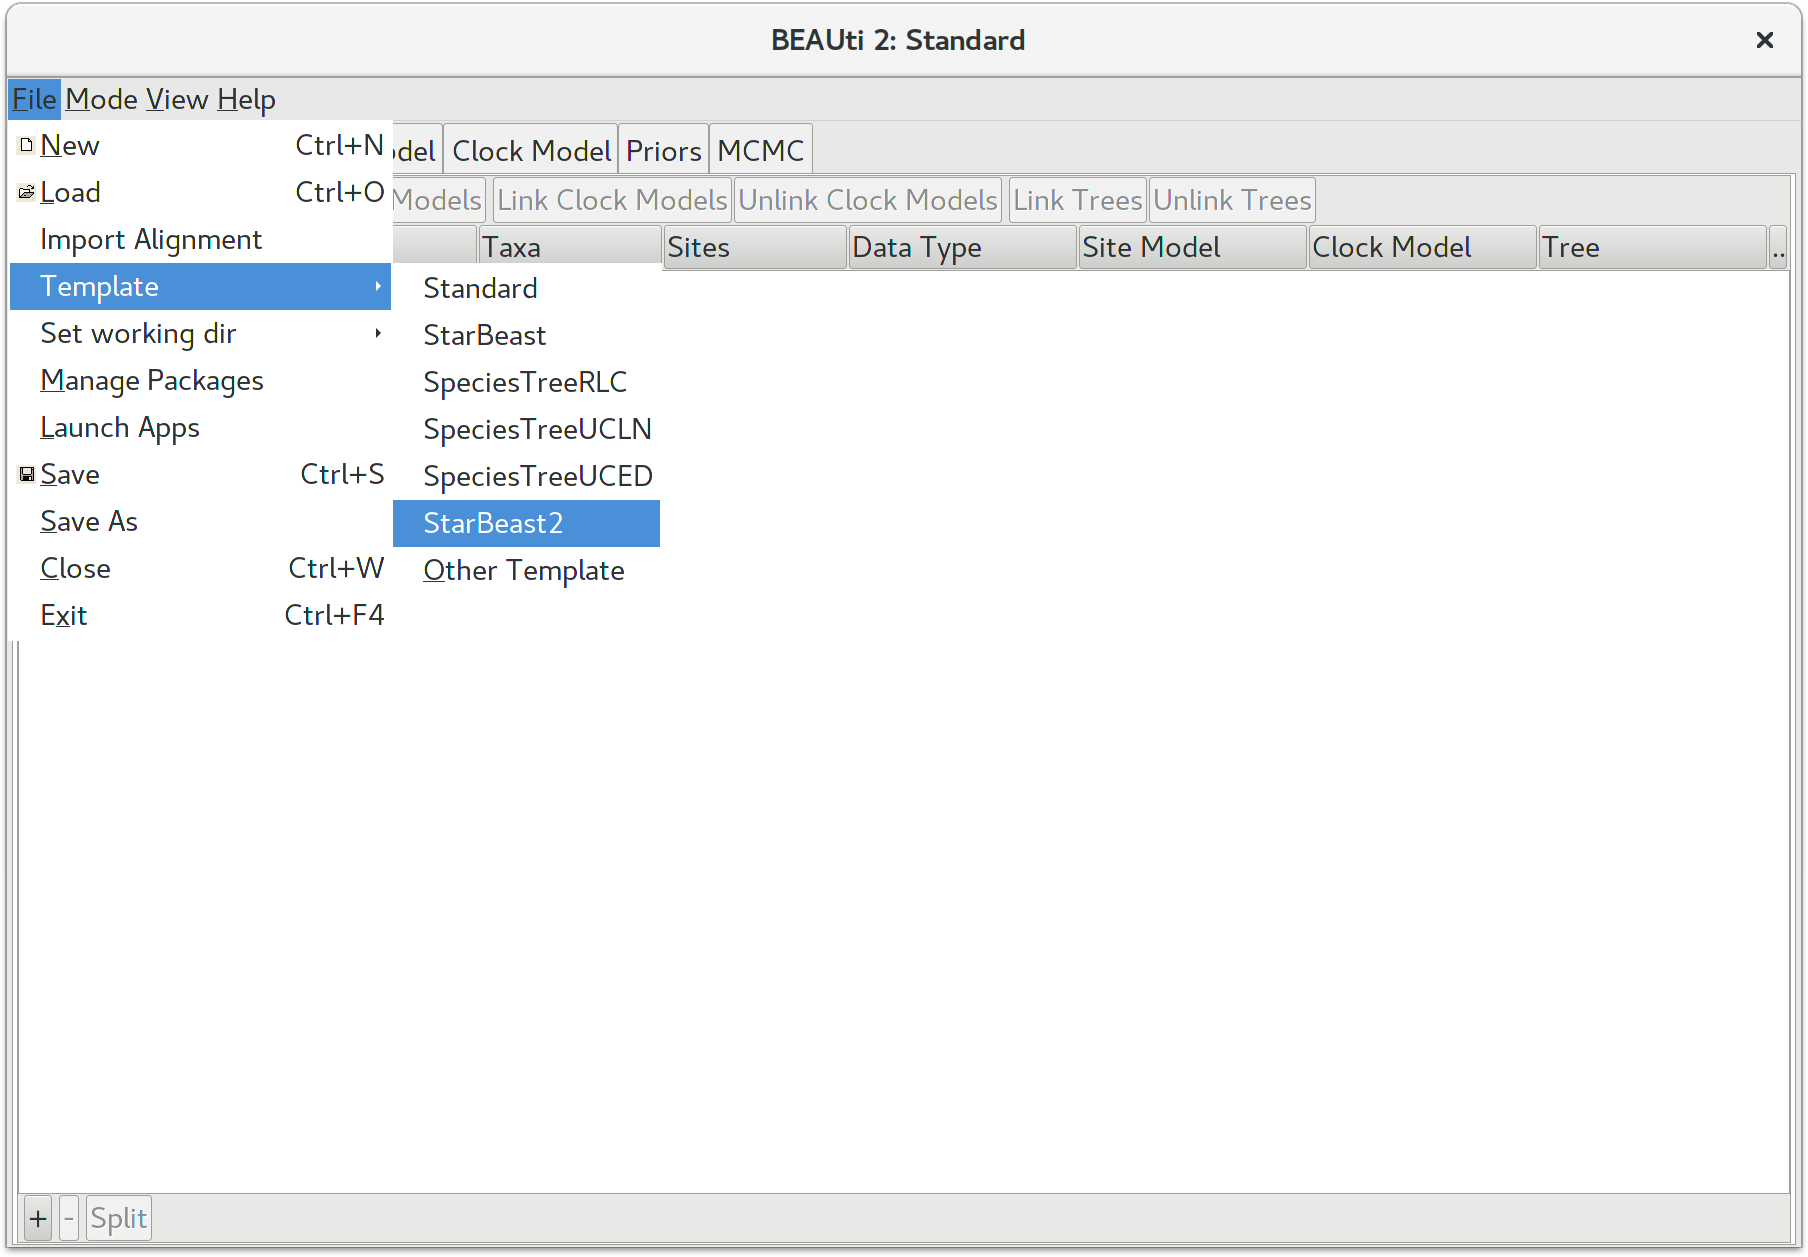
\includegraphics[width=\textwidth]{figures/beauti-strict.png}
\caption{Select a species tree template in BEAUti.}
\label{fig:sb2Template}
\end{figure}

\clearpage

\subsubsection*{Allow clock rates to vary}

By default BEAUTi fixes the clock rate of the first partition to 1, so that
the rates of other loci are estimated relative to the first locus. This is
generally inappropriate for StarBEAST2 analyses, so it is \textcolor{red}{very
important} to disable this behaviour by deselecting the \textbf{Mode/Automatic
set clock rate} menu item (Figure~\ref{fig:disableAuto}).

\begin{figure}[htb!]
\centering
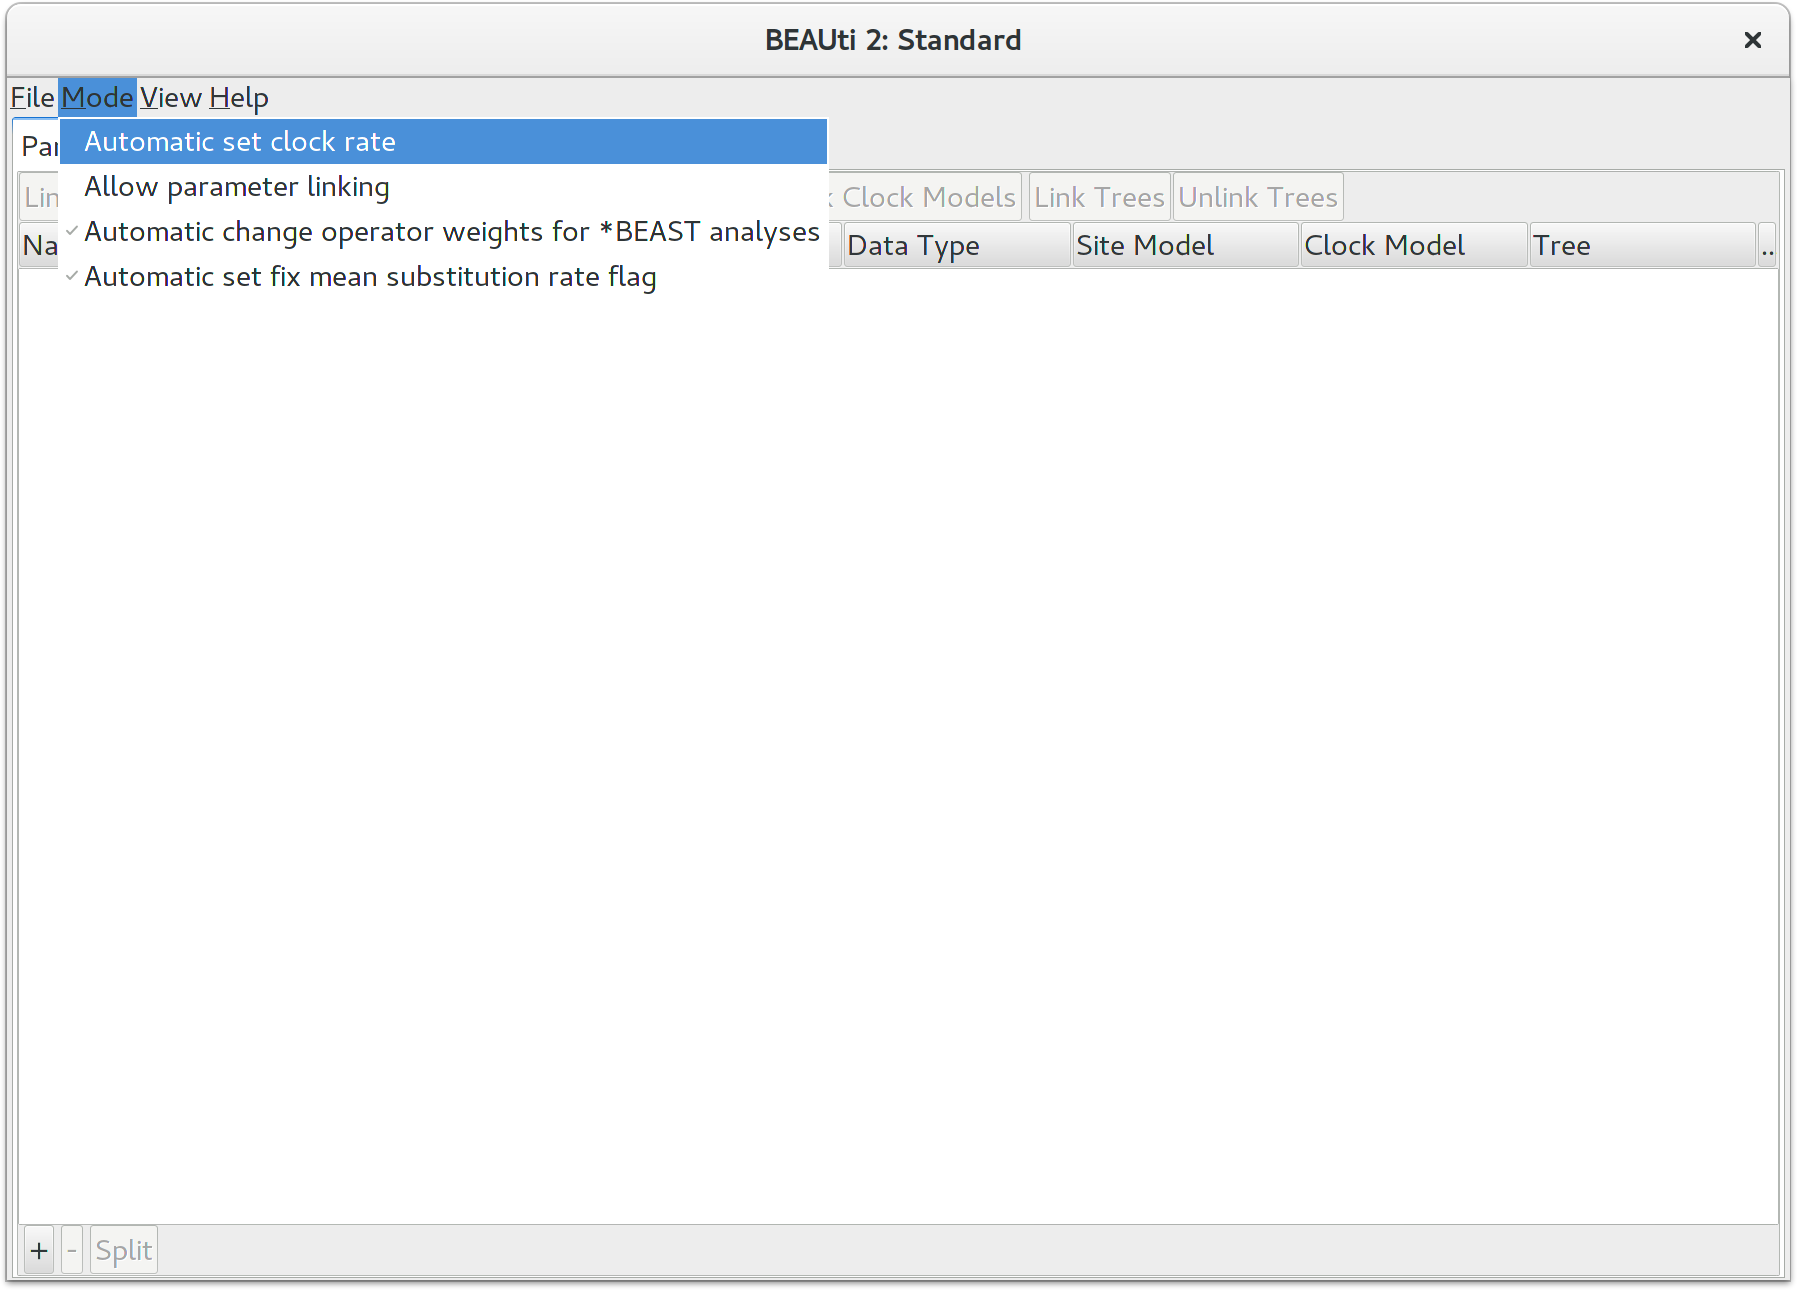
\includegraphics[width=\textwidth]{figures/beauti-disable.png}
\caption{Disable automatic setting of clock rates.}
\label{fig:disableAuto}
\end{figure}

\clearpage

\subsubsection*{Loading the NEXUS files}

To load a NEXUS format alignment, click the button with the plus symbol ($+$) in
the lower left corner of the main \textbf{Partitions} tab. We will be using the
same sequence files as in the previous tutorial;
navigate to the \textbf{examples/nexus} subfolder inside the \textbf{beast}
application folder, and select all of the first seven NEXUS files. They should
be numbered 26, 29, 47, 53, 59, 64, and 72 (Figure~\ref{fig:importAlignments}).

\begin{figure}[htb!]
\centering
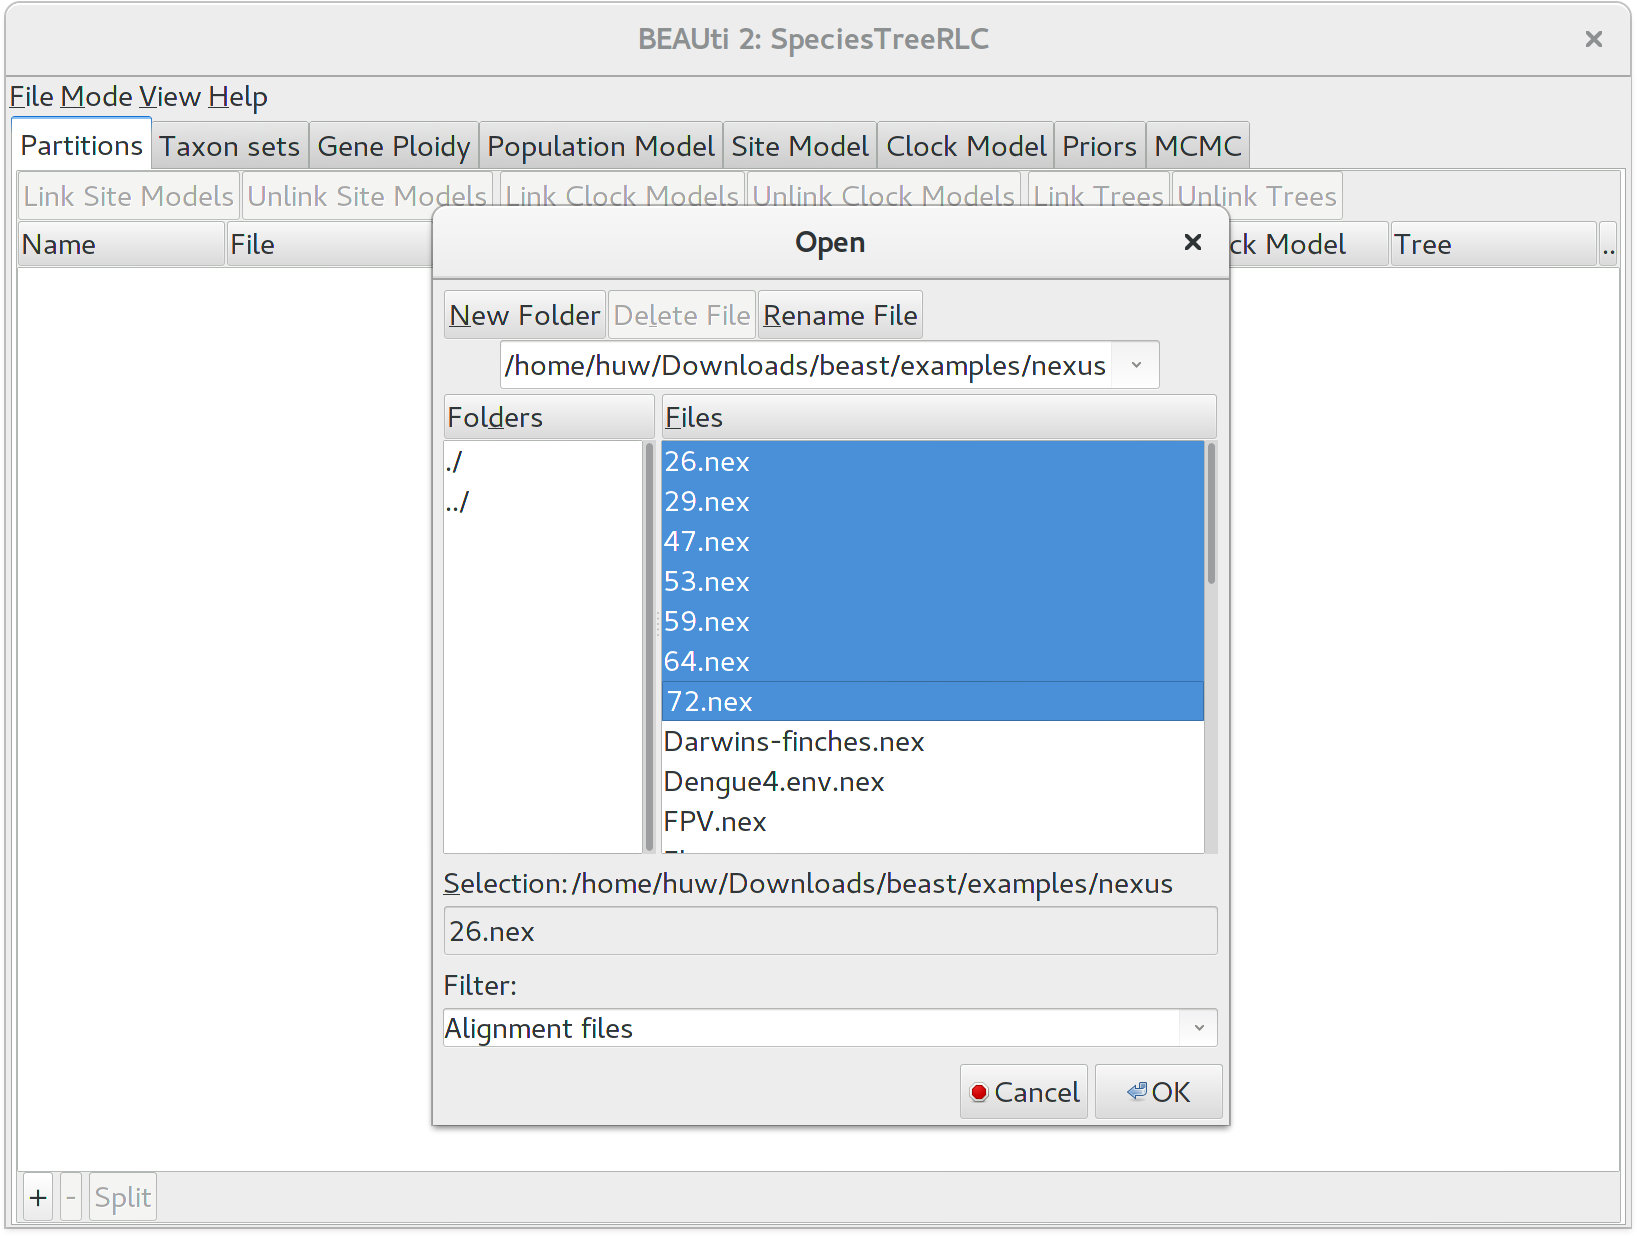
\includegraphics[width=\textwidth]{figures/beauti-import.png}
\caption{Selecting NEXUS alignment files to import.}
\label{fig:importAlignments}
\end{figure}

\clearpage

\subsubsection*{Assigning the correct species to each sequence}

As in the previous tutorial, splitting the name on the underscore character
`\_' and selecting the second group will give us the mapping that we need
(Figure~\ref{fig:taxonSets}).

\begin{figure}[htb!]
\centering
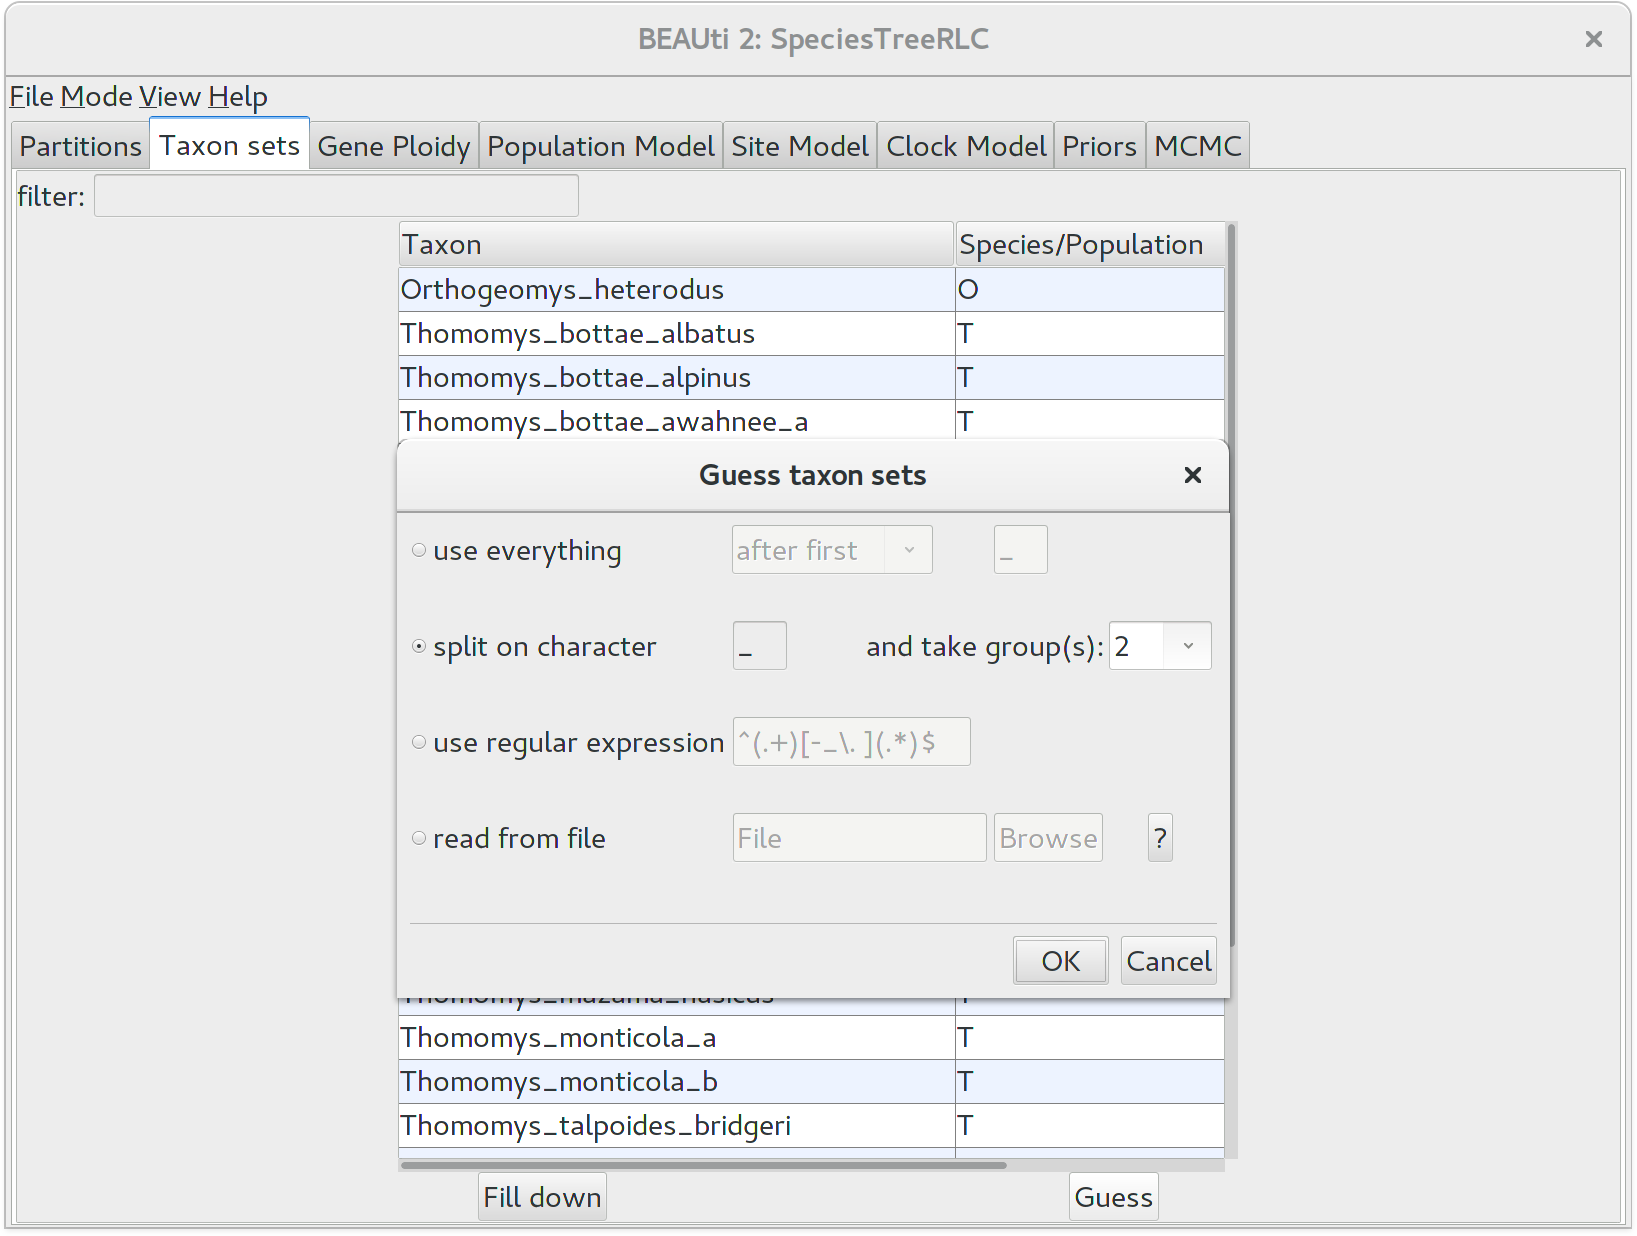
\includegraphics[width=\textwidth]{figures/beauti-guess.png}
\caption{Assigning species to sequences in BEAUti using the guess dialog.}
\label{fig:taxonSets}
\end{figure}

\clearpage

\subsubsection*{Ploidy and population models}

As in the previous tutorial, leave the ploidy of each gene and the
population model at their default values.

\subsubsection*{Setting the substitution model}

For this tutorial we will also use the HKY substitution model, but will use a
shortcut to set it for all genes at once. For the first gene (which should be
``26'') select ``HKY'' for substitution model (\textbf{Subst Model} in
Figure~\ref{fig:HKY}) Now select the other six genes using the shift key. The
right panel will now allow you to set the same substitution model for
those six genes by cloning the parameters from the first gene. Click \textbf{OK}
to proceed (Figure~\ref{fig:clone}).

\begin{figure}[htb!]
\centering
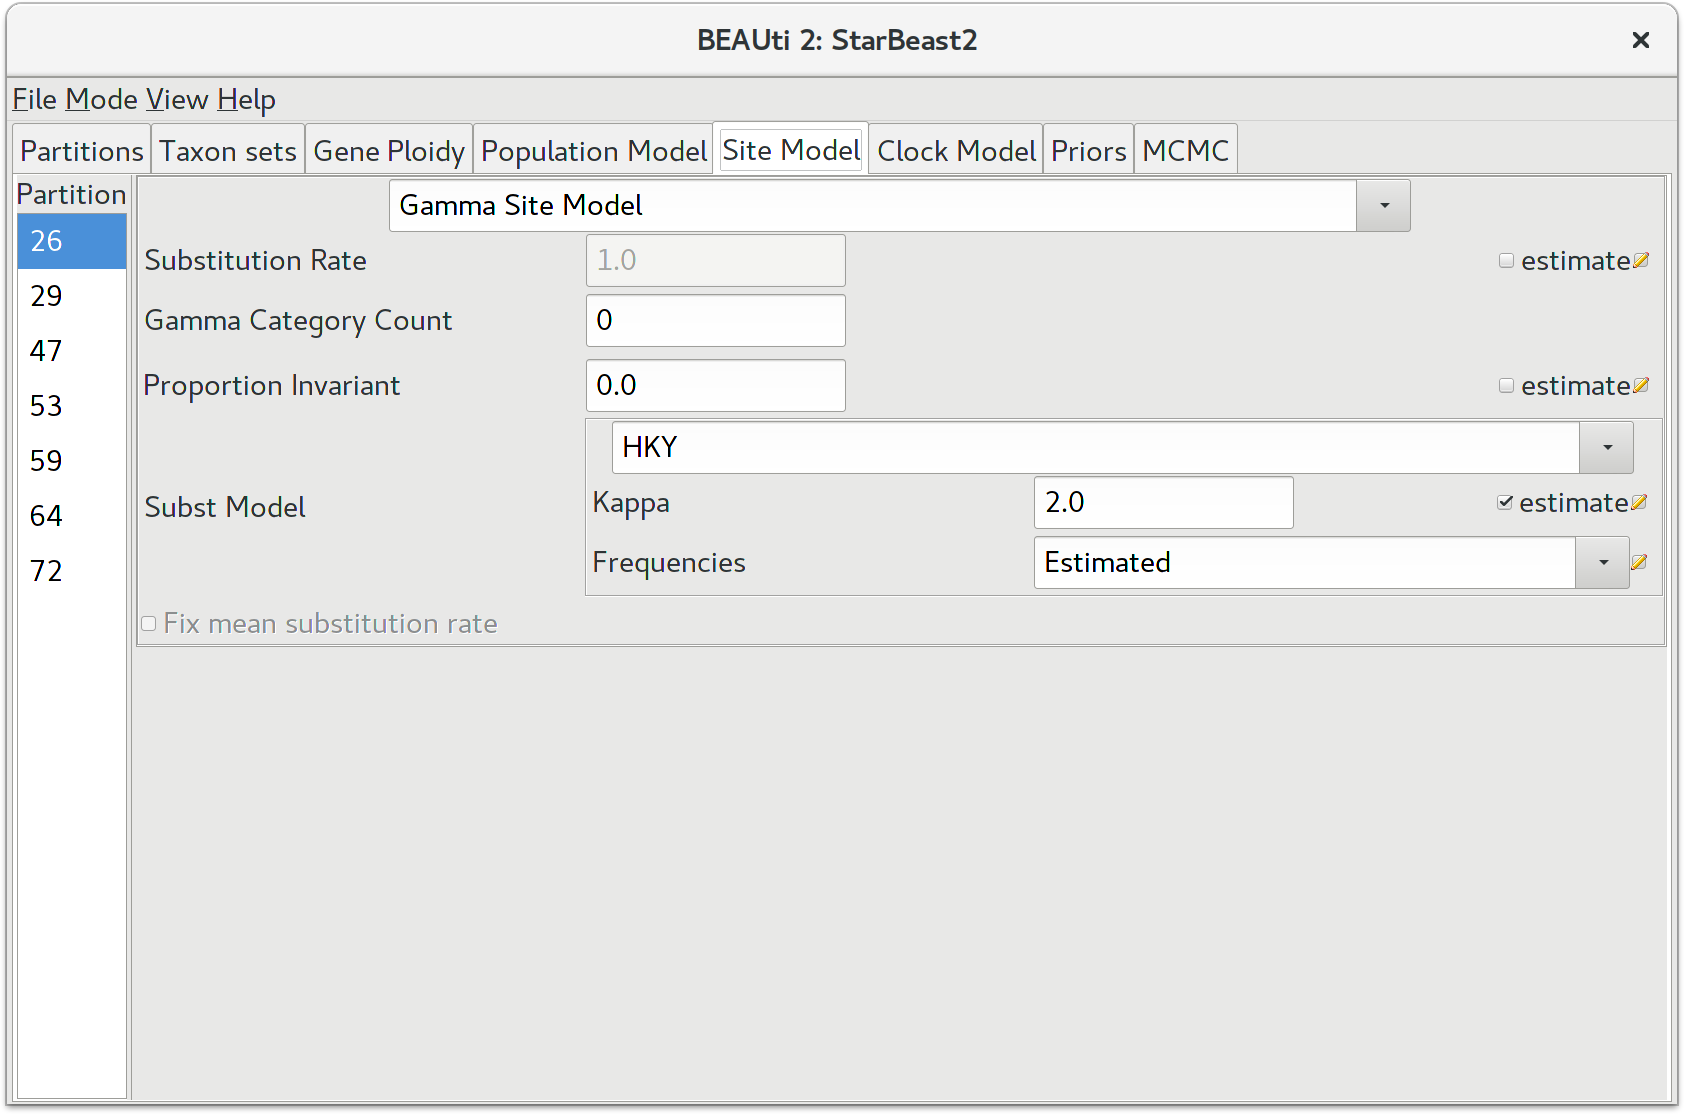
\includegraphics[width=\textwidth]{figures/beauti-hky.png}
\caption{Setting up substitution and site models for the gopher alignments.}
\label{fig:HKY}
\end{figure}

\begin{figure}[htb!]
\centering
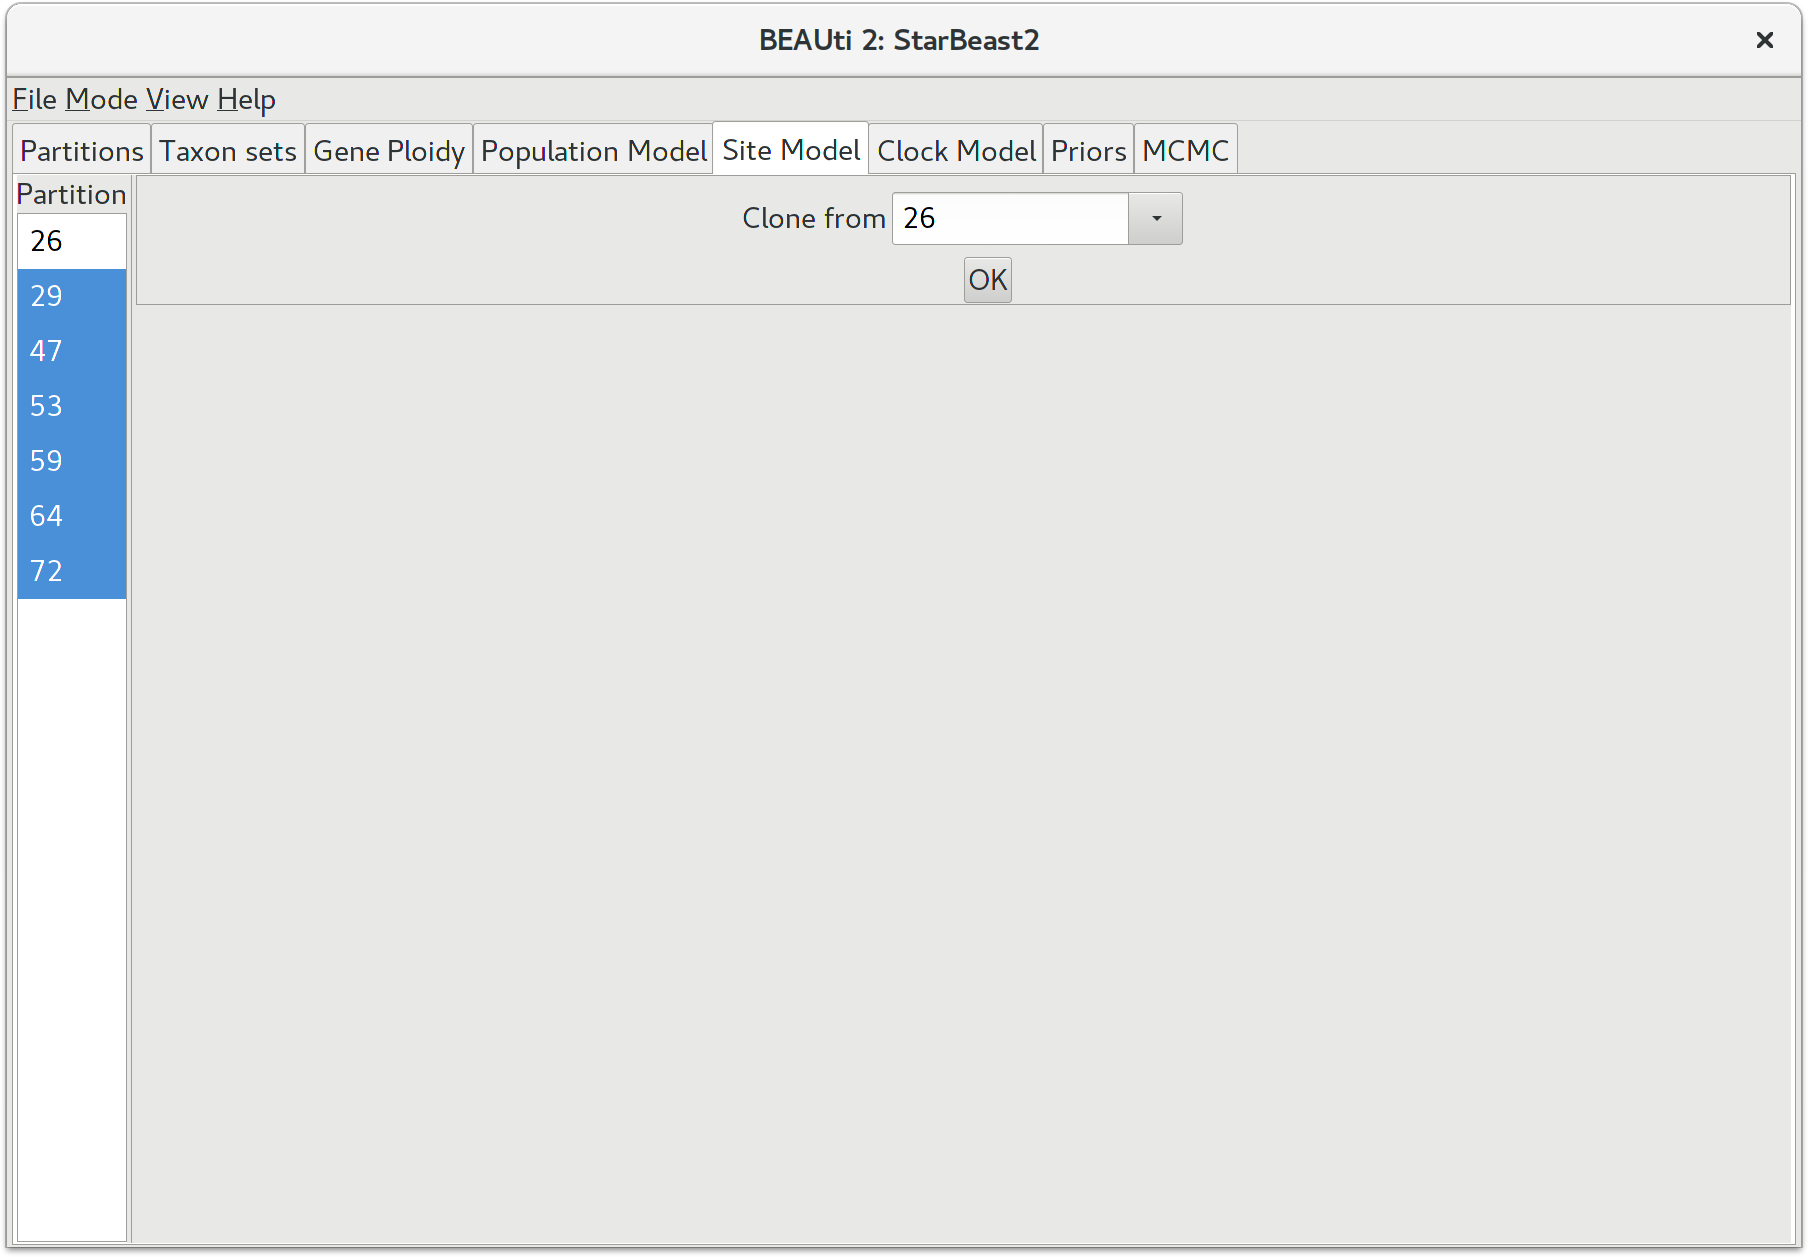
\includegraphics[width=\textwidth]{figures/beauti-clone.png}
\caption{Setting multiple substitution and site models at once.}
\label{fig:clone}
\end{figure}

\clearpage

\subsubsection*{Setting the clock model}

Click on the \textbf{Clock Model} tab at the top of the main window. In this
panel you can configure the mean clock rate for each locus. If you followed the
earlier instructions to disable automatic setting of clock rates, the
mean clock rate ``Clock.rate'' of all partitions should have the
\textbf{estimate} box ticked (Figure~\ref{fig:clock}).

\begin{figure}[htb!]
\centering
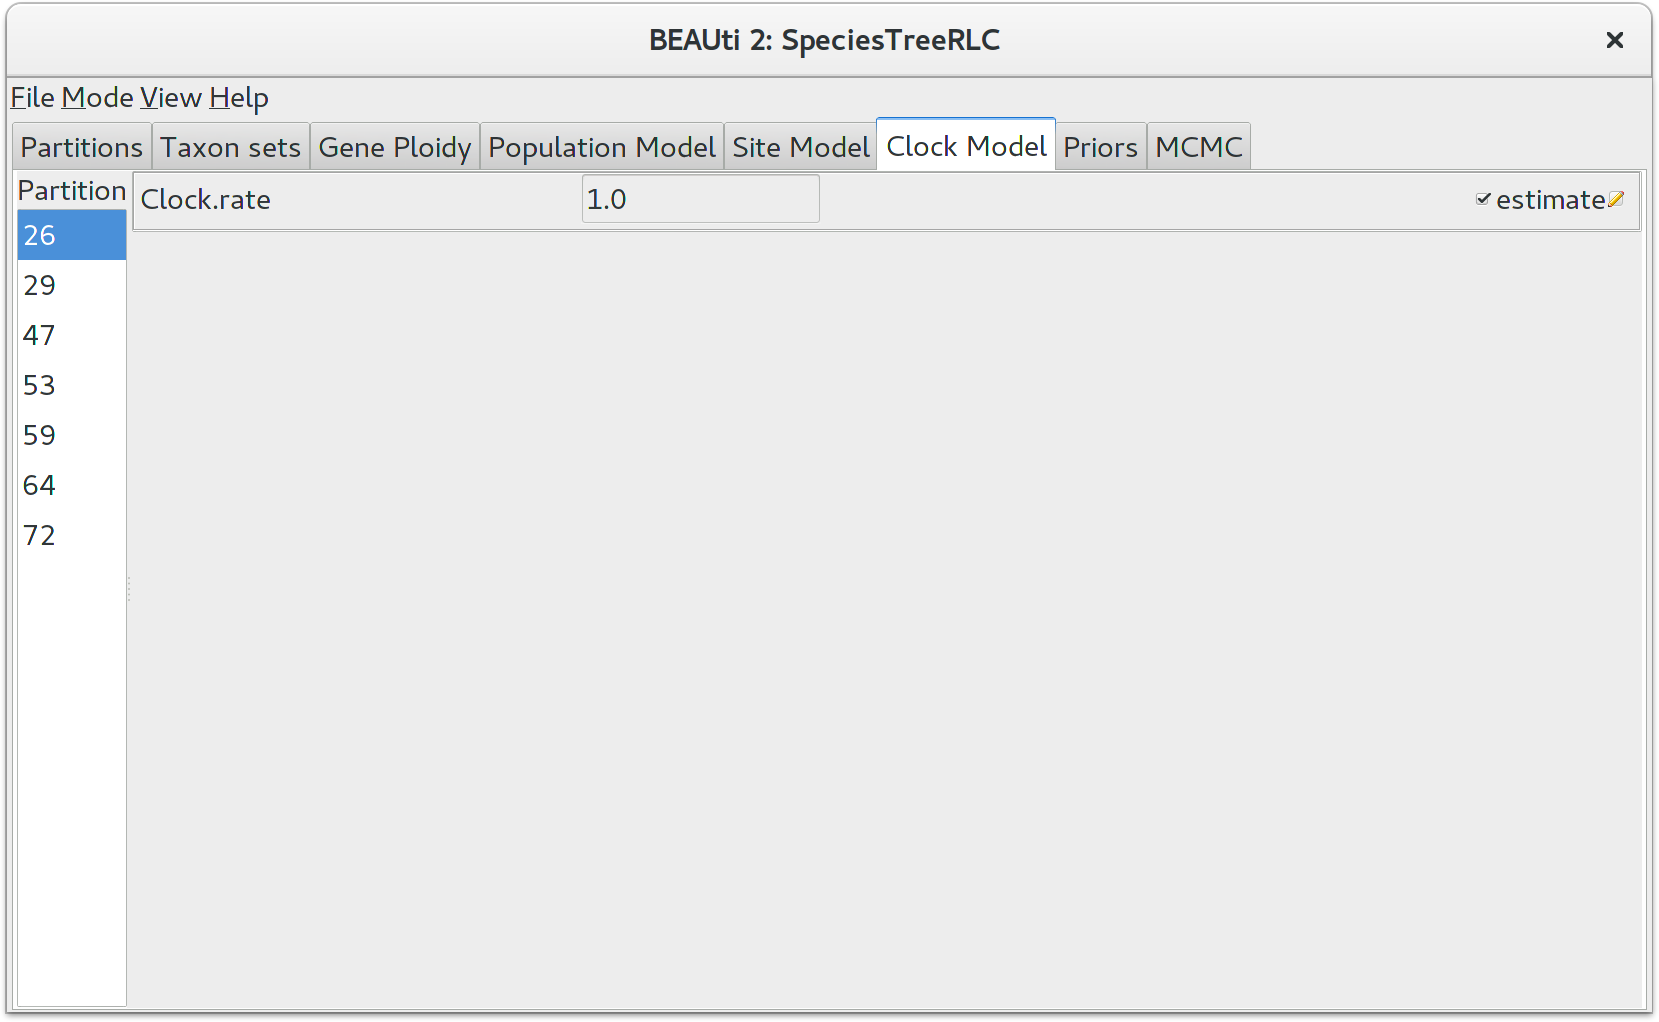
\includegraphics[width=\textwidth]{figures/beauti-clock.png}
\caption{The default when automatic clock rate setting is disabled.}
\label{fig:clock}
\end{figure}

\clearpage

\subsubsection*{Priors}

Before applying the date calibration first change the prior on the species
tree, ``Tree.t:Species'', to \textbf{calibrated Yule} \citep{Heled01012012}.
Click the top-leftmost arrow to expand the options available for the
calibrated Yule model, leave the Birth Rate at 1.0, and uncheck the
\textbf{estimate} box to make this a fixed parameter. \textcolor{red}{For real
analyses you should almost certainly estimate this value, but a fixed value
will help us complete the tutorial in a reasonable time frame.}

The default prior for mean clock rates in StarBEAST2 is a lognormal
distribution with a mean (in real space) of 1. This will not be appropriate
when using fossil (or other external) calibrations. For this tutorial we will
use the 1/X prior, which is uninformative and will allow the calibration(s) to
guide the clock rates. For each clockRate.c:\textit{gene} parameter, set
the prior distribution to be 1/X (Figure~\ref{fig:jeffreys})

\begin{figure}[htb!]
\centering
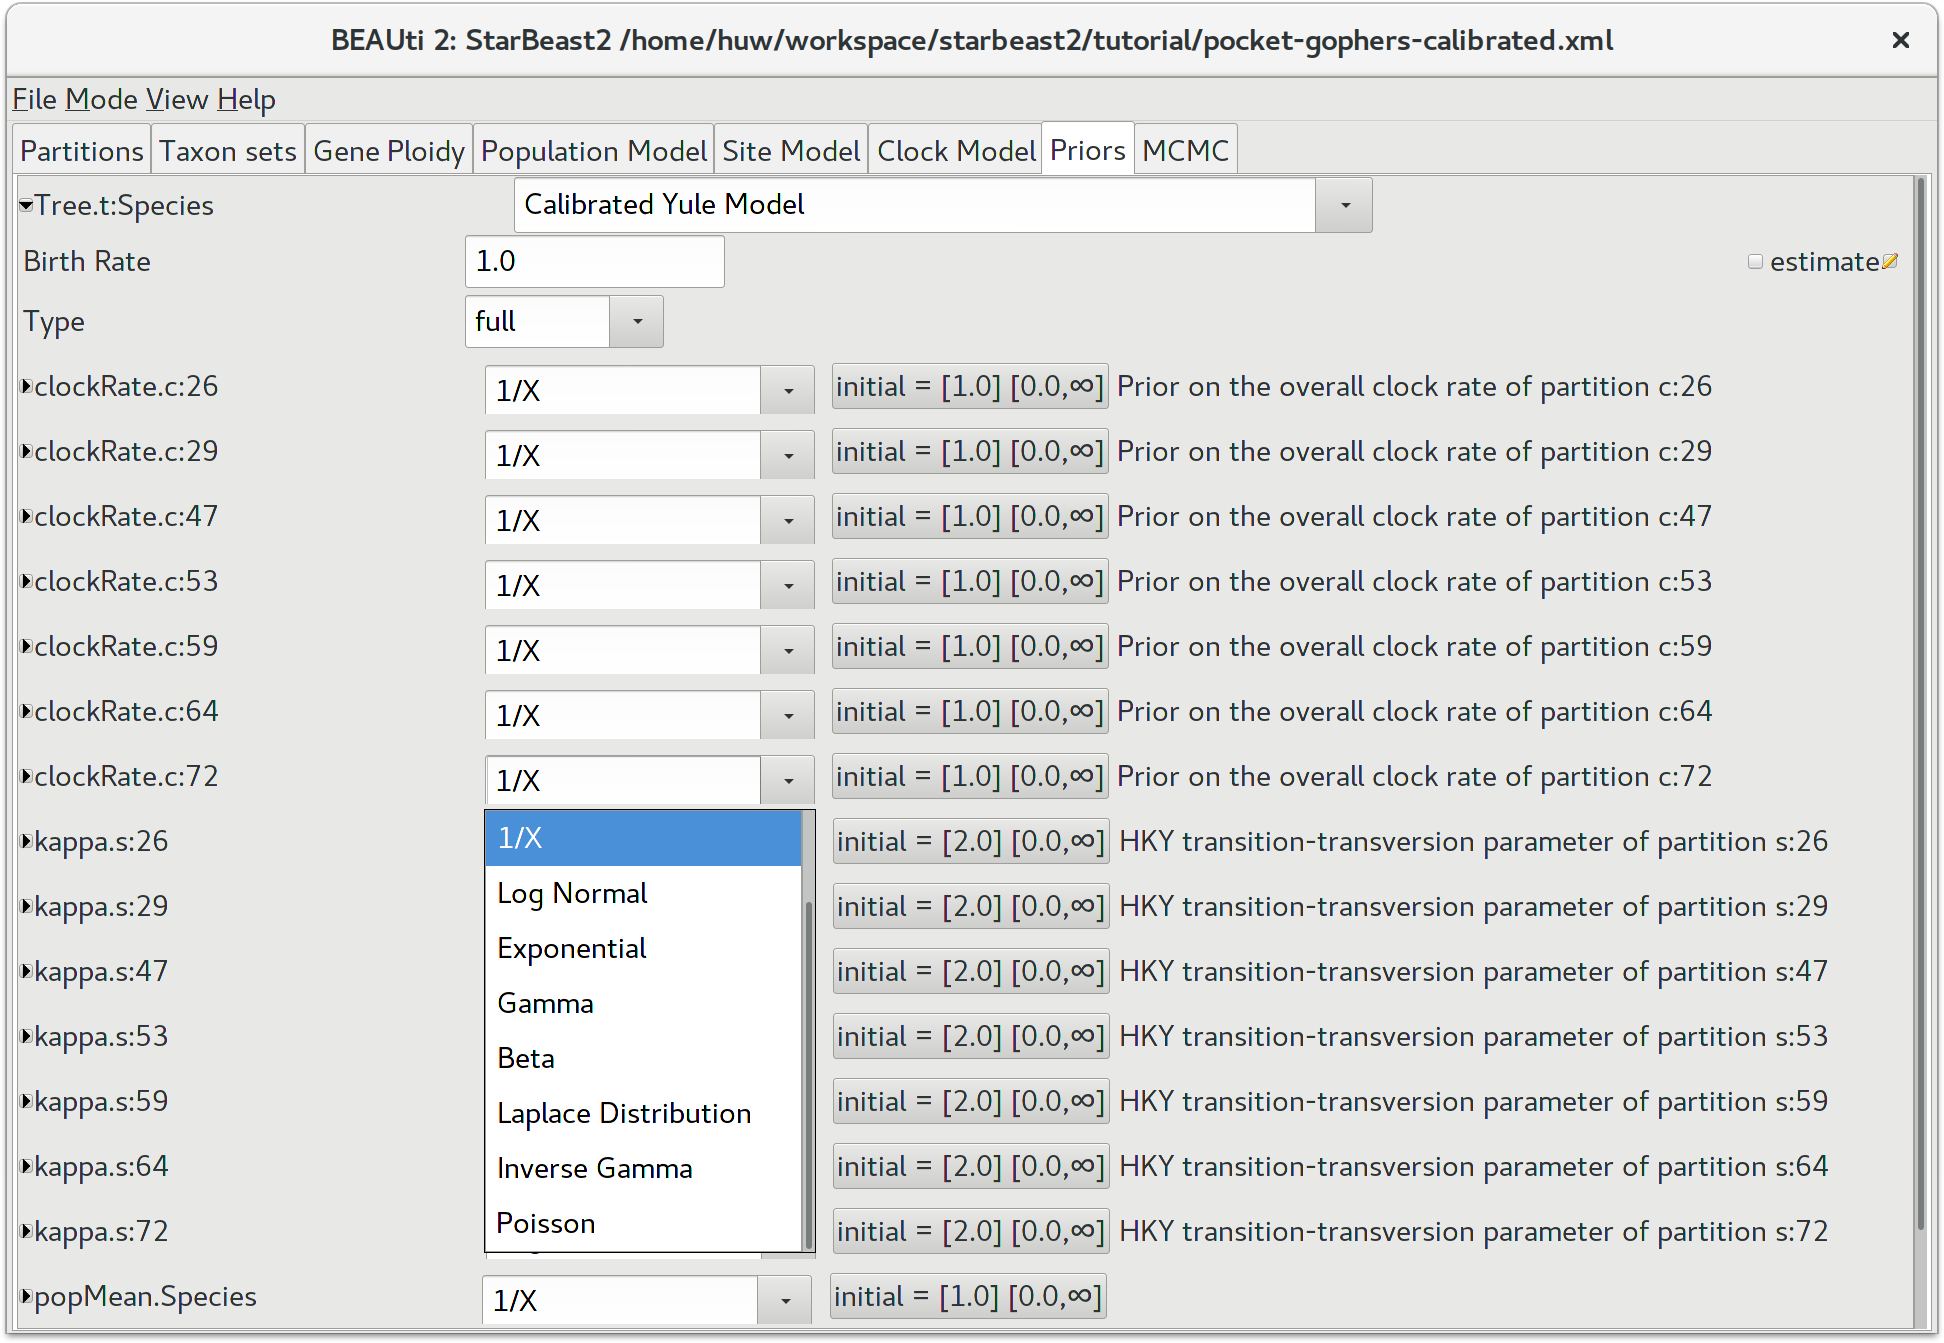
\includegraphics[width=\textwidth]{figures/beauti-jeffreys.png}
\caption{Setting an uninformative prior on clock rates.}
\label{fig:jeffreys}
\end{figure}

We can calibrate this analysis by applying a date calibration to the root of
the species tree. This is equivalent to the split between
\textit{Thomomys} and \textit{Orthogeomys}, estimated to have occured between
6.5ma and 6.8ma \citep{Belfiore01042008}.

To add the new date calibration, click the button with the plus symbol ($+$)
at the very bottom of the list of priors, and click OK to add a new MRCA (most
recent common ancestor) prior. Select ``Tree.t:Species'' to apply this prior
to the species tree.

Because this prior applies to the root node, move all the species from the left
hand column to the right hand column using the $>>$ button. Give this taxon set
a sensible name, for example ``root'' (Figure~\ref{fig:mrca-taxonset}).

\begin{figure}[htb!]
\centering
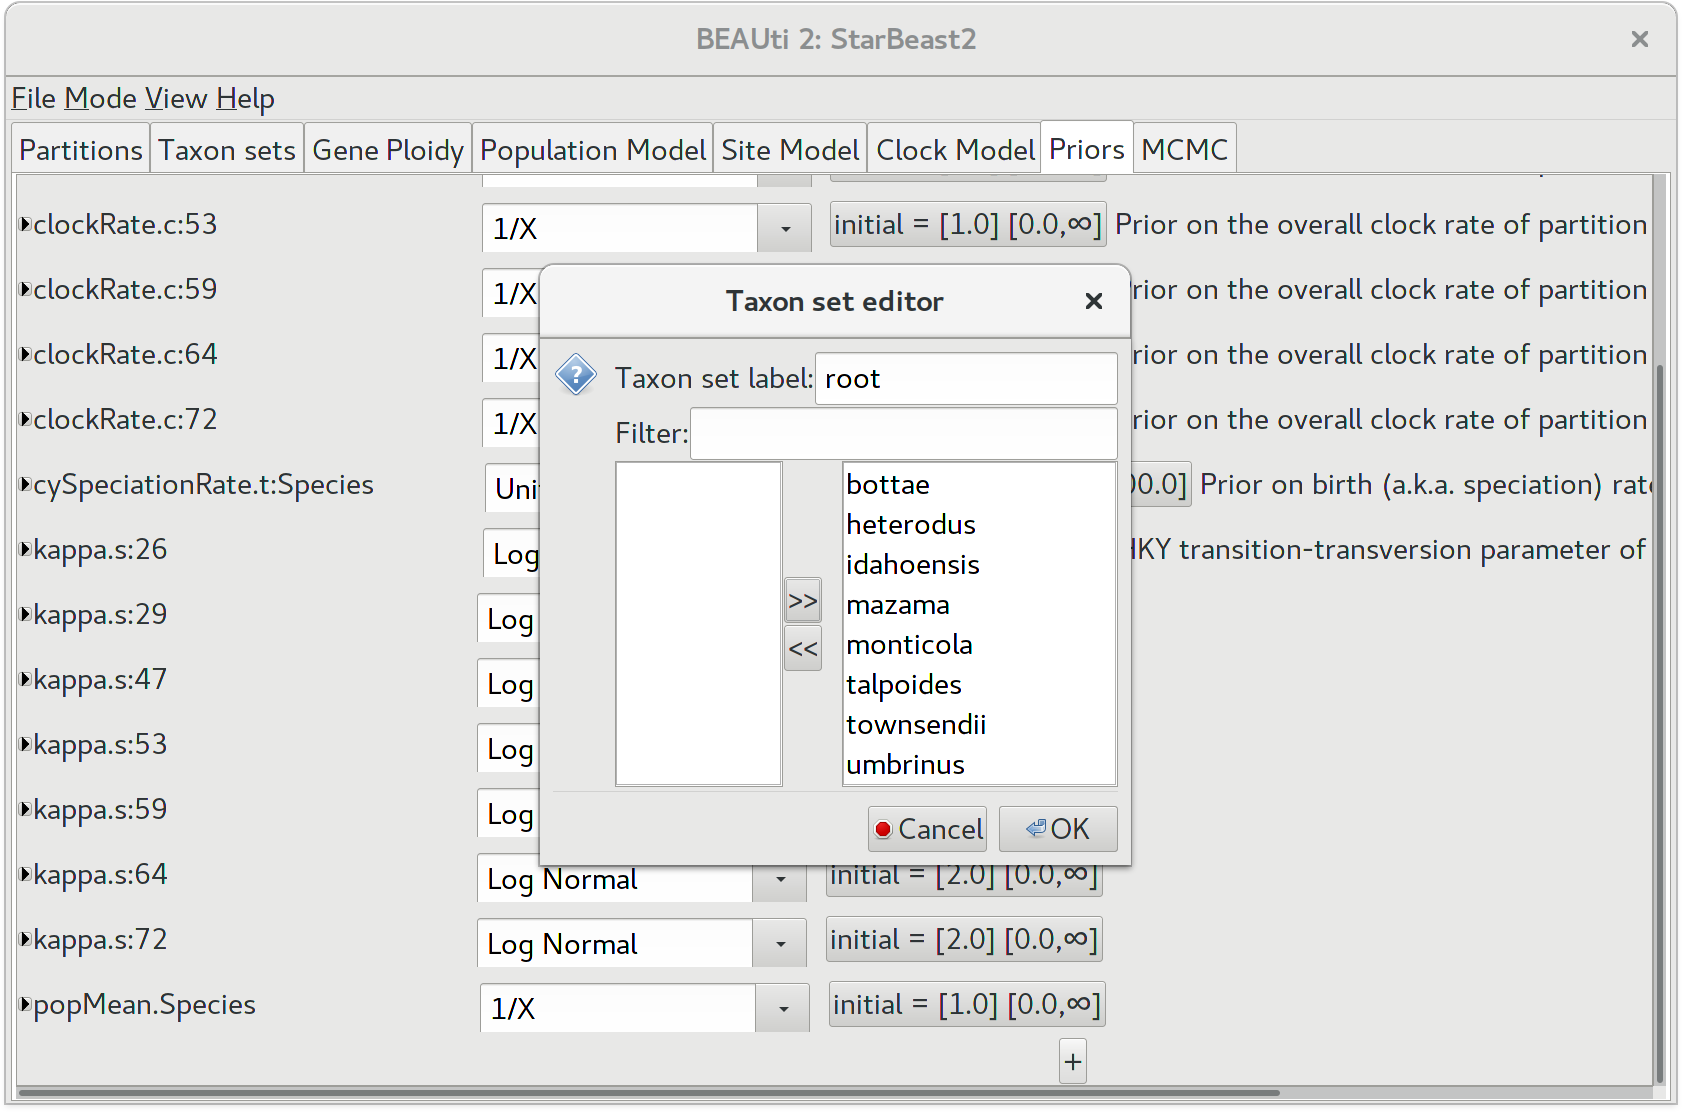
\includegraphics[width=\textwidth]{figures/beauti-mrca-taxonset.png}
\caption{Setting an uninformative prior on clock rates.}
\label{fig:mrca-taxonset}
\end{figure}

Make this prior monophyletic by checking the ``monophyletic'' tick box. If
6.5ma is a lower bound, we can use an exponential prior with an offset of 6.5
to set a lower limit on the root node height. Set the mean of the exponential
distribution to 0.15, so that the mean of the prior is equal to 6.65ma, the
midpoint of the estimated range (Figure~\ref{fig:mrca-prior}).

\begin{figure}[htb!]
\centering
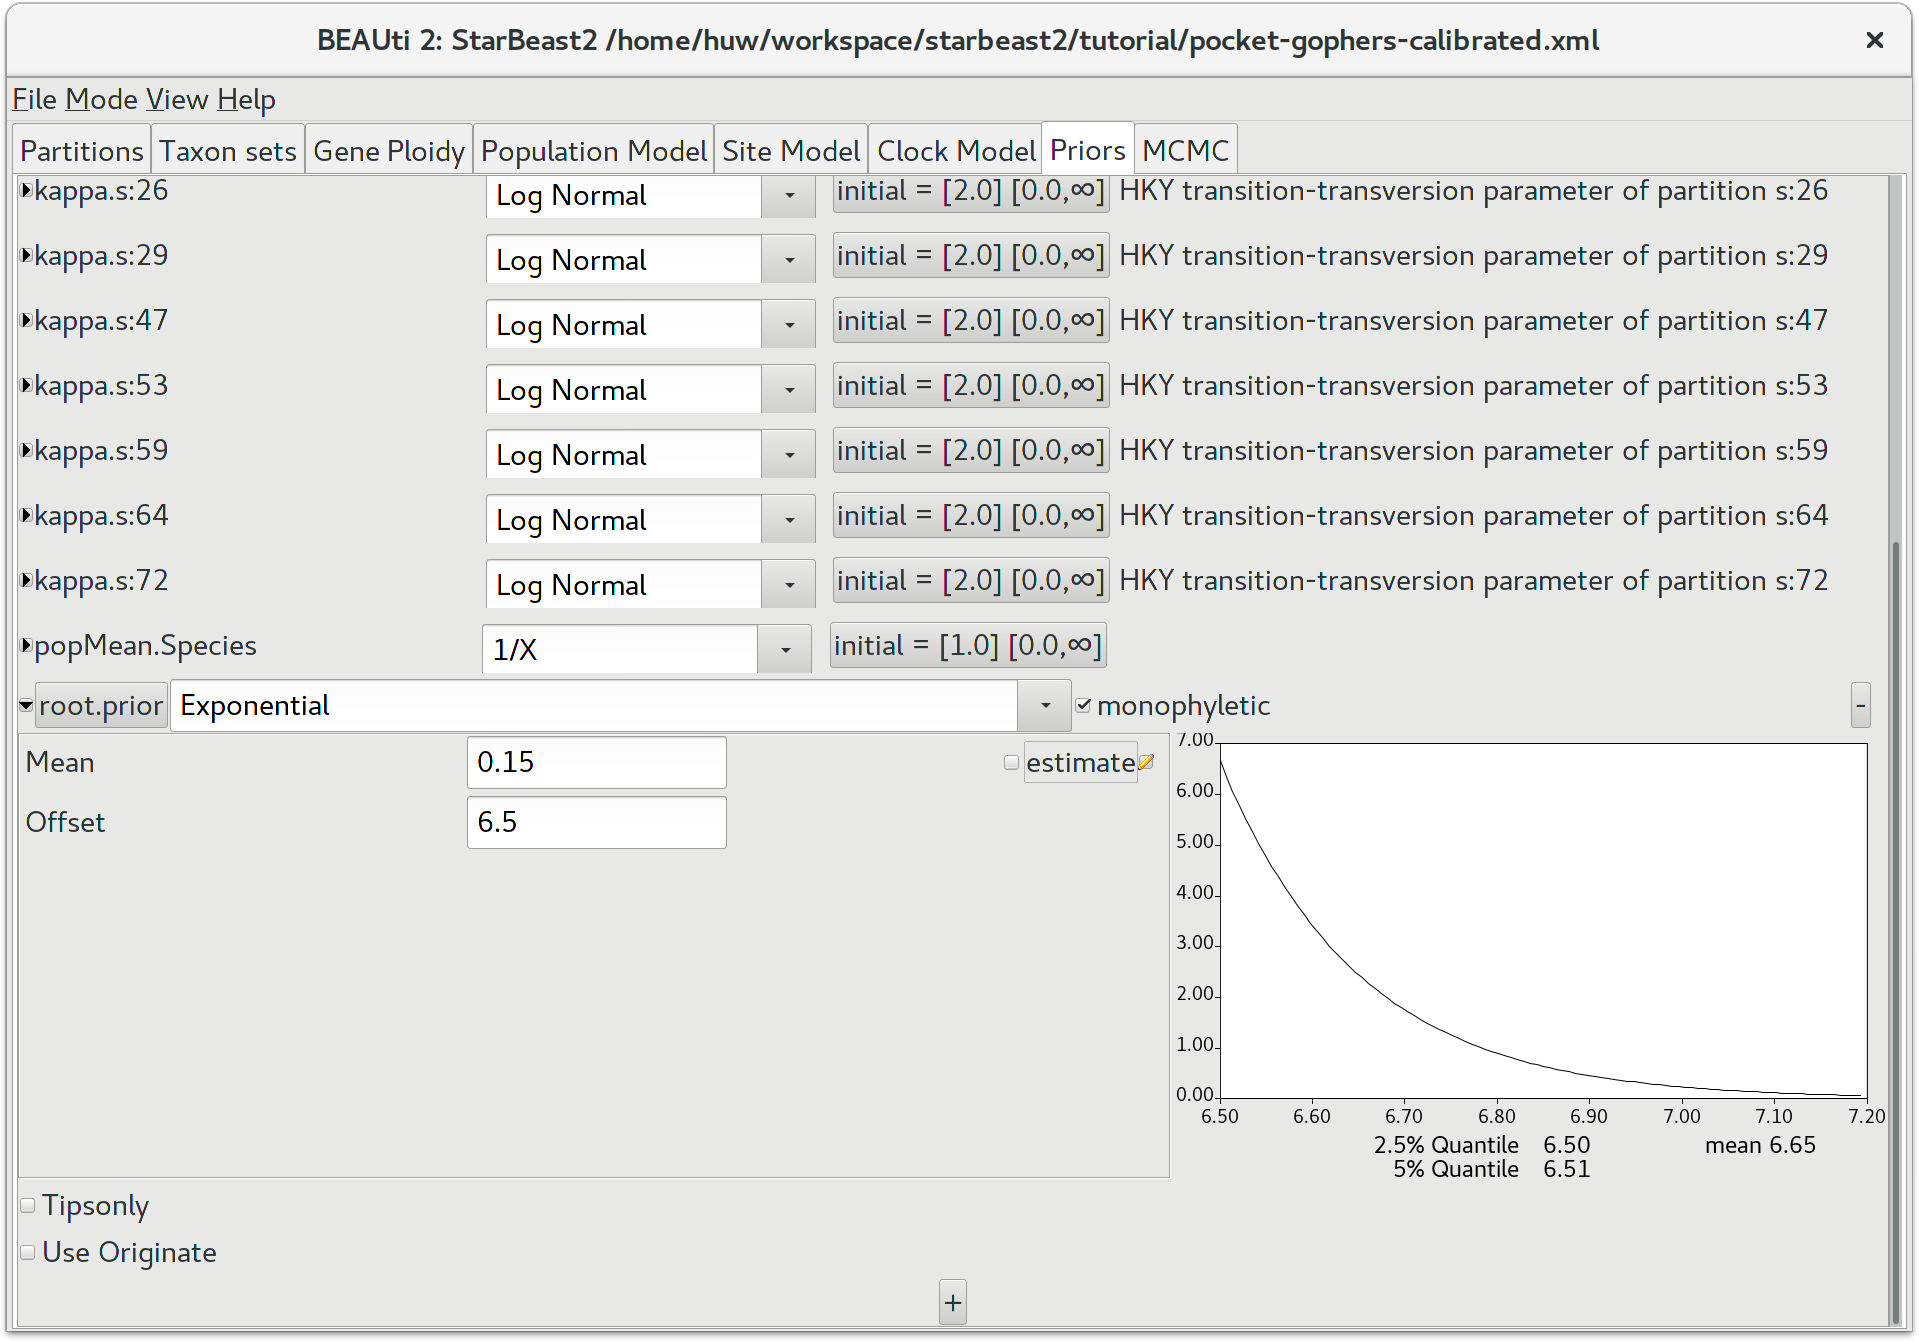
\includegraphics[width=\textwidth]{figures/beauti-mrca-prior.png}
\caption{Setting an uninformative prior on clock rates.}
\label{fig:mrca-prior}
\end{figure}

\subsubsection*{Generating the BEAST XML file}

As in the previous tutorial, stick to the default settings in the MCMC tab.
We are now ready to create the BEAST XML file. To do this, either select the
\textbf{File/Save} or \textbf{File/Save~As} menu options. Save the file with an
appropriate name (we usually end the filename with ``.xml'', e.g.
``pocket-gophers-calibrated.xml''). We are now ready to run the file through BEAST.

\subsection*{Running BEAST}

Now run BEAST and when it asks for an input file, provide your newly created XML
file as input by clicking \textbf{Choose~File...}, and then click \textbf{Run}.
In Linux BEAST will immediately launch a file opening dialog box, which is to
select the BEAST XML to run. BEAST will then run until it has finished reporting
information to the screen. The actual results files are saved to the disk in the
same location as your input file.

\section{Analyzing the results}

Run the program called \textbf{Tracer} to analyze the output of BEAST. When the
main window has opened, choose \textbf{Import Trace File...} from the
\textbf{File} menu and select the file that BEAST has created called
``starbeast.log''. Select the clock rates for all genes using the shift key,
then click on the ``Marginal Prob Distribution'' tab.
You should now see a window like in Figure~\ref{fig:tracer}.

\begin{figure}[htb!]
\centering
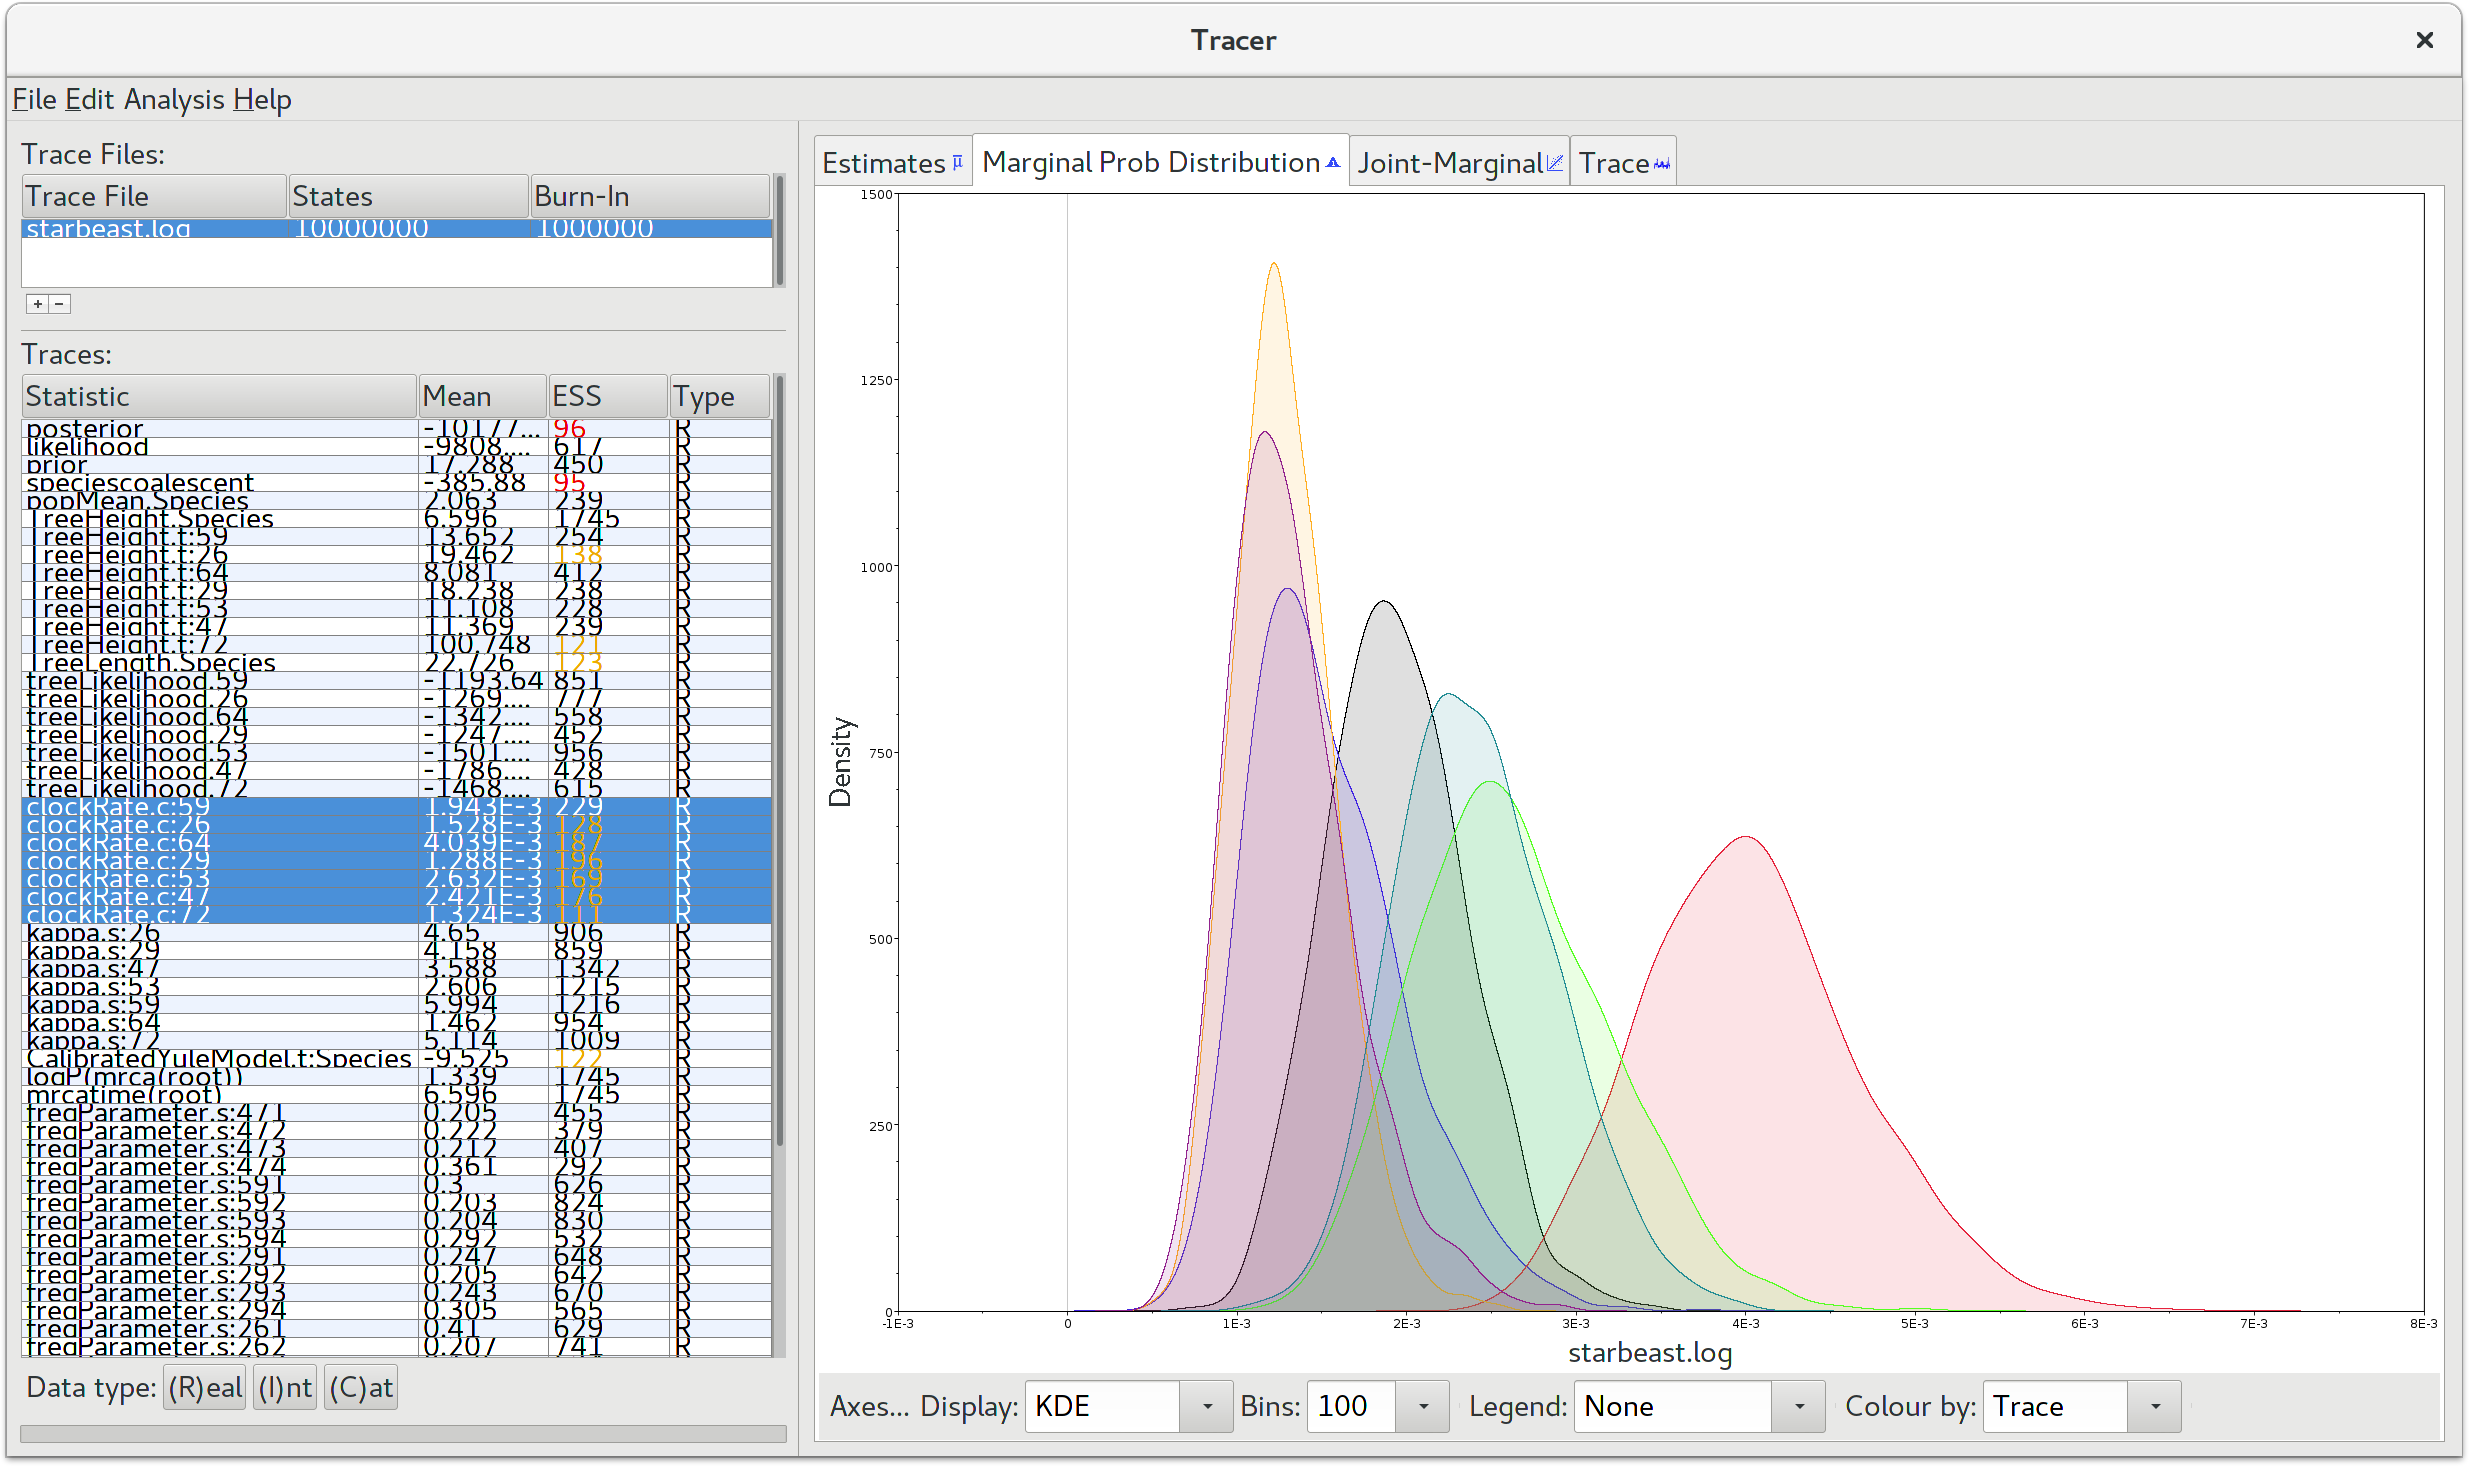
\includegraphics[width=\textwidth]{figures/tracer-clock-rates.png}
\caption{Tracer with the gopher data.}
\label{fig:tracer}
\end{figure}

This display shows the marginal distributions of clock rates for all loci.
Remember that MCMC is a stochastic algorithm so the actual distributions will
not be exactly the same. The clock rates (in units of substitutions per million years) range from about 0.001 for genes 29
and 72 to 0.004 for locus 64, demonstrating that the loci sequenced by
\cite{Belfiore01042008} have slower and faster rates of molecular evolution
respectively.

\clearpage

\subsection*{Obtaining an estimate of the phylogenetic tree}

Summarize the posterior sample produced by BEAST by running the
\textbf{TreeAnnotator} program and setting it up to look like in
Figure~\ref{fig:treeannotator}.

\begin{figure}[htb!]
\centering
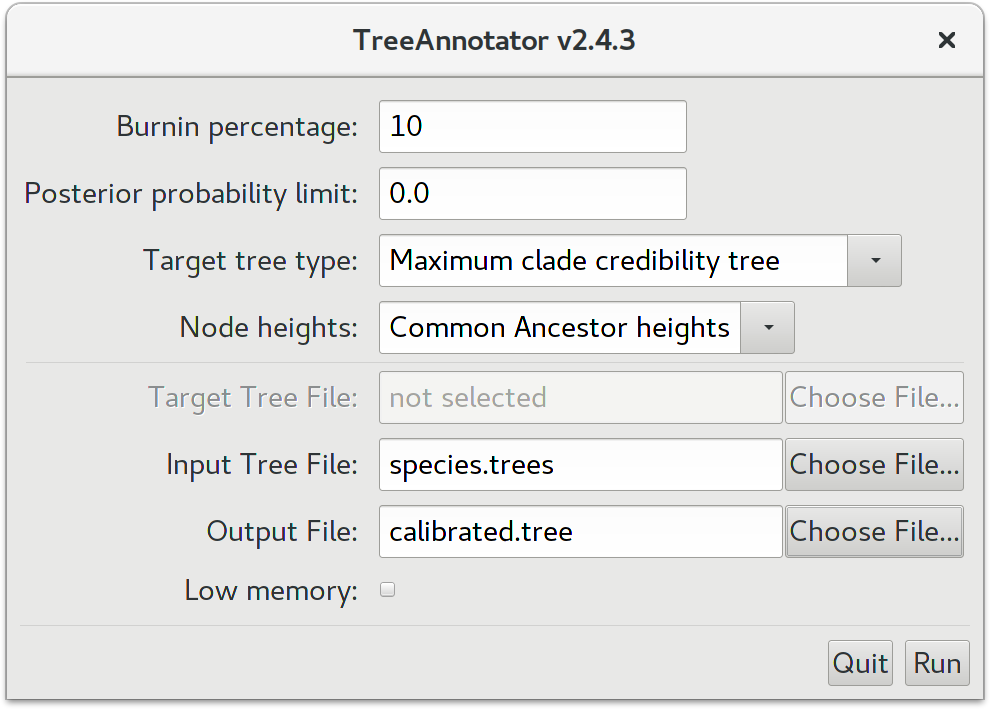
\includegraphics[width=0.7\textwidth]{figures/treeannotator-calibrated.png}
\caption{Using TreeAnnotator to summarise the tree set.}
\label{fig:treeannotator}
\end{figure}

The \textbf{Burnin percentage} is the proportion of trees to remove from the
start of the sample; for this tutorial, set a 10\% burnin as shown in
Figure~\ref{fig:treeannotator}.

The \textbf{Posterior probability limit} option specifies a limit such that if a
node is found at less than this frequency in the sample of trees (i.e., has a
posterior probability less than this limit), it will not be annotated.

For \textbf{Target tree type} you can either choose a specific tree from a file
or ask TreeAnnotator to find a tree in your sample. The default option,
\textbf{Maximum clade credibility tree}, finds the tree with the highest product
of the posterior probability of all its nodes.

Keep ``Common Ancestor heights'' for \textbf{Node heights}. This sets the
heights (ages) of each node in the tree to the mean height of the most recent
common ancestor across the entire set of trees in the posterior.

For the input file, select the trees file that BEAST created (by default this
will be called ``species.trees'') and select a file for the output (here we
have called it ``calibrated.tree''). Now press \textbf{Run} and wait for the
program to finish.

\clearpage

\subsection*{Viewing the species tree(s)}

Run \textbf{FigTree} and open the ``calibrated.tree'' file by using the
Open command in the File menu. The tree should appear. Select \textbf{Node
Bars} to get node age error bars. Disable \textbf{Scale Bar} and select
\textbf{Scale Axis} to indicate the ages when speciation events occured. You
should end up with something like Figure \ref{fig:figtree}.

\begin{figure}[htb!]
\centering
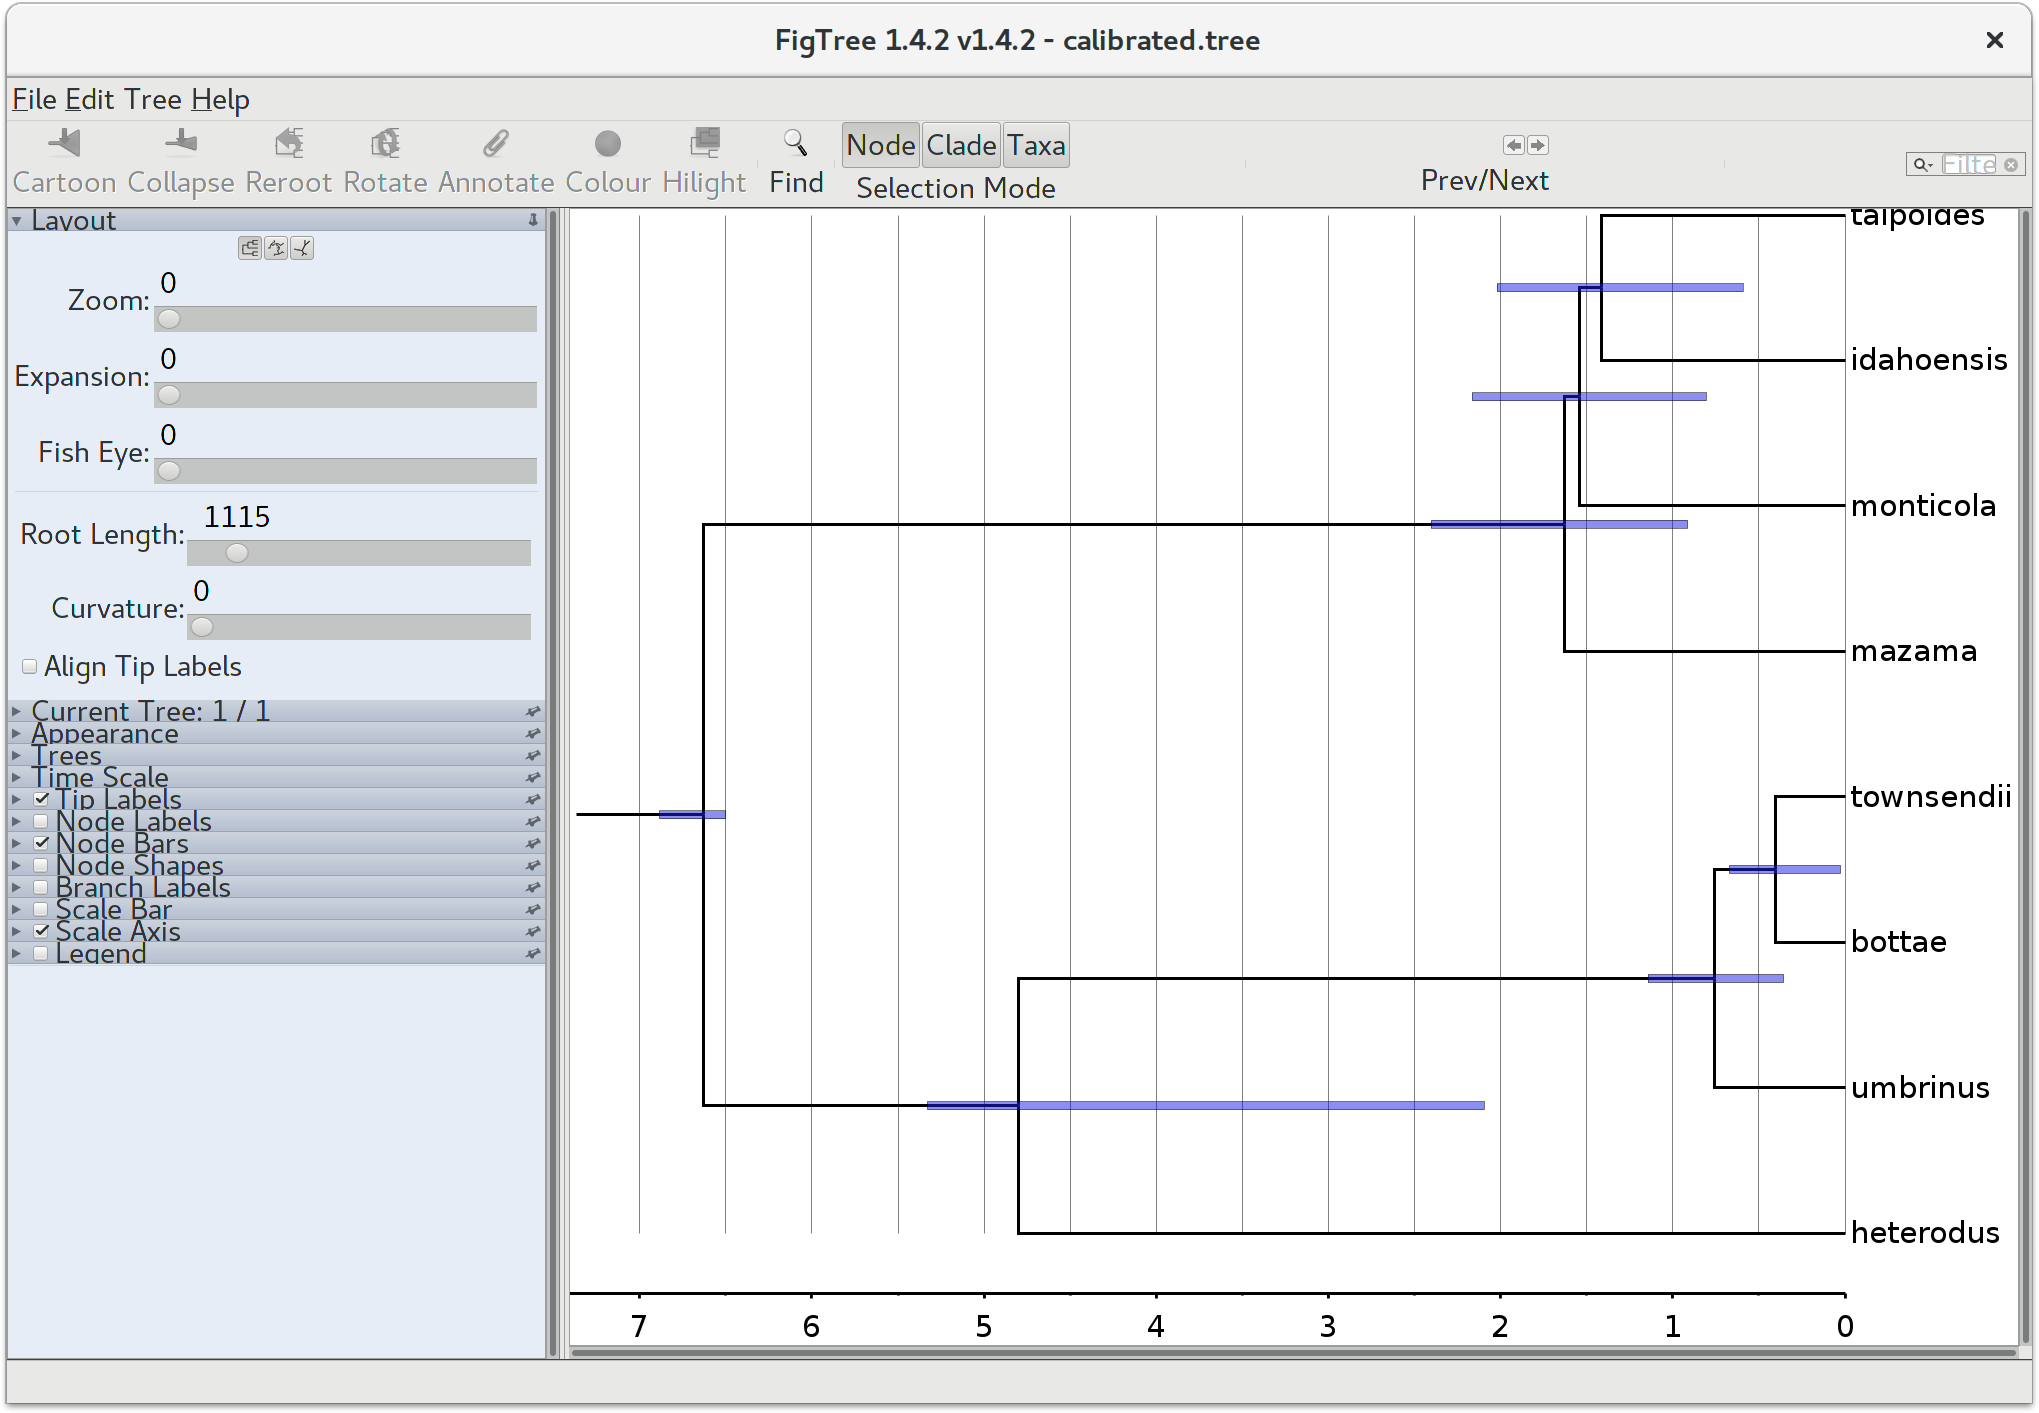
\includegraphics[width=\textwidth]{figures/figtree-calibrated.png}
\caption{Figtree representation of the species tree.}
\label{fig:figtree}
\end{figure}

According to our reanalysis, the radiation of \textit{T. townsendii},
\textit{T. bottae}, and \textit{T. umbrinus} occured quite recently, within
the last million years. On the other hand timing of the \textit{T. heterodus}
split is uncertain, and could have occured more than 5ma or as recently as 2ma.

\clearpage

%%%%%%%%%%%%%%%%%%%%%%%
% Tutorial disclaimer %
%%%%%%%%%%%%%%%%%%%%%%%
% Please do not change the license
% Add the author names and relevant links
% Add any other aknowledgments here
\href{http://creativecommons.org/licenses/by/4.0/}{
\includegraphics[scale=0.8]{figures/ccby.pdf}} This tutorial was written by Huw A. Ogilvie for \href{https://taming-the-beast.github.io}{Taming the BEAST} and is licensed under a \href{http://creativecommons.org/licenses/by/4.0/}{Creative Commons Attribution 4.0 International License}. 


%%%%%%%%%%%%%%%%%%%%
% Do NOT edit this %
%%%%%%%%%%%%%%%%%%%%
Version dated: \today



\newpage

%%%%%%%%%%%%%%%%
%  REFERENCES  %
%%%%%%%%%%%%%%%%

\printbibliography[heading=relevref]


\end{document}